\documentclass[xcolor={usenames,dvipsnames,svgnames,table}]{beamer}

\mode<presentation>
\usetheme{Madrid}

\usecolortheme[RGB={80,0,0}]{structure}
\useoutertheme[subsection=false]{miniframes}
\useinnertheme{default}

% hide navigation controlls
\setbeamertemplate{navigation symbols}{}

\setbeamercolor{normal text}{fg=black}
\setbeamercovered{dynamic}
\beamertemplatetransparentcovereddynamicmedium
%\usepackage{chronology}
\setbeamertemplate{caption}[numbered]

\definecolor{Maroon}{RGB}{80,0,0}
\definecolor{BurntOrange}{RGB}{204,85,0}

% load macros and prevent authblk from loading
\makeatletter
% prevent a package from loading
\newcommand{\dontusepackage}[2][]{%
    \@namedef{ver@#2.sty}{9999/12/31}%
    \@namedef{opt@#2.sty}{#1}
}

% a macro to load packages only if they are not yet loaded, needed for combination of beamer and hyperref
\newcommand{\usepackagesave}[2][{}]{
    \ltx@ifpackageloaded{#2}{}{
        \usepackage[#1]{#2}}
}
\makeatother
\dontusepackage{authblk}

% load packages, settings and definitions
% this file contains all commonly used packages for the Rattlesnake documentation
% new package, add comment what they are used for

% command packages
\usepackage{xifthen}     % if -then else command

% language and font improvements
\usepackage[english]{babel}	% Multilingual support - https://www.ctan.org/pkg/babel
\usepackage[utf8]{inputenc} % Accept different input encodings - https://www.ctan.org/pkg/inputenc
\usepackage[kerning,spacing,babel]{microtype} % Subliminal refinements towards typographical perfection - https://www.ctan.org/pkg/microtype
\usepackage{eepic}      % Extensions to epic - https://www.ctan.org/pkg/eepic
\usepackage{epic}       % Enhance LaTeX picture mode - https://www.ctan.org/pkg/epic
\usepackage[T1]{fontenc} % selecting font encodingsselecting font encodings - https://www.ctan.org/pkg/fontenc
\usepackage{lmodern}

% title packages
\usepackage{authblk}		% footnote style author/affiliation - https://www.ctan.org/pkg/authblk

% symbols
\usepackage{upgreek}		% Upright Greek letters - https://www.ctan.org/pkg/upgreek
\usepackage{cancel}			% \cancel cmd - https://www.ctan.org/pkg/cancel

% chemical and isotope packages
\usepackage{isotope}		% isotope command - https://www.ctan.org/pkg/isotope
\usepackage{mhchem}			% chemical formulae/equations - https://www.ctan.org/pkg/mhchem

% layout packages
\usepackage{xspace}			% smart space \xspace - https://www.ctan.org/pkg/xspace
\usepackage{icomma}			% smart math comma - https://www.ctan.org/pkg/icomma
\usepackage{chngpage}		% page layout change during document - https://www.ctan.org/pkg/chngpage
\usepackage[usenames,dvipsnames,svgnames,table]{xcolor}			% color definitions - https://www.ctan.org/pkg/xcolor
\usepackage{enumitem}   % layout for itemize and enumerate - http://www.ctan.org/pkg/enumitem
\usepackage{setspace}    % allows for \singlespacing, \onehalfspacing, and \doublespacing commands - https://www.ctan.org/pkg/setspace

% floating packages
% needed by the breakalgo environment labelsep=quad
\usepackage[singlelinecheck=false, labelsep=quad]{caption}	% table captions - https://www.ctan.org/pkg/caption
\usepackage{subcaption}		% Support for sub-captions - https://www.ctan.org/pkg/subcaption
\usepackage{placeins}   	% Control float placement - https://www.ctan.org/pkg/placeins
\usepackage{float}      	% Improved interface for floating objects - https://www.ctan.org/pkg/float

% table packages
\usepackage{supertabular}	% multi-page tables package - https://www.ctan.org/pkg/supertabular
\usepackage{booktabs}		% table settings - https://www.ctan.org/pkg/booktabs
\usepackage{array}			% Extending the array and tabular environments - https://www.ctan.org/pkg/array
\usepackage{multirow}		% tabular cells spanning multiple rows - https://www.ctan.org/pkg/multirow
% \usepackage{tabls}      % Better vertical spacing in tables and arrays - https://www.ctan.org/pkg/tabls
\usepackage{colortbl}      % Allows for color manipulation within tables - https://www.ctan.org/pkg/colortbl

% pictures, plots and listings
\usepackage{graphicx}		% include graphics - https://www.ctan.org/pkg/graphicx
\usepackage{wrapfig}		% wrapfigure enviroment - https://www.ctan.org/pkg/wrapfig
\usepackage{pgfplots}		% latex plots - https://www.ctan.org/pkg/pgfplots


% source code and algorithms
\usepackage{algorithmicx} % newer version of algorithmic - https://www.ctan.org/pkg/algorithmicx
\usepackage{listings} 	% source code listings - http://www.ctan.org/pkg/listings
\usepackage{verbatim}   % verbatim - https://www.ctan.org/pkg/verbatim

% misc packages
\usepackage{url}        % provide \url command for web addresses - https://www.ctan.org/pkg/url
\usepackage{import}			% Establish input relative to a directory - https://www.ctan.org/pkg/import
\usepackage{afterpage}  % Execute command after the next page break - https://www.ctan.org/pkg/afterpage
\usepackage{lscape}     % Place selected parts of a document in landscape - https://www.ctan.org/pkg/lscape
\usepackage{rotating}   % Rotation tools, including rotated full-page floats - https://www.ctan.org/pkg/rotating
\usepackage{chngcntr}   % Change the resetting of counters - http://ctan.org/pkg/chngcntr
\usepackage{textpos}    % Allows logo and banner manipulation

% eps support
\usepackage{epsfig}       % include eps figures - https://www.ctan.org/pkg/epsfig
\usepackage{epsf}          % Simple macros for EPS inclusion - https://www.ctan.org/pkg/epsf
\usepackage{epstopdf}   %use .eps images (as pdf) in \includegraphics


% reference packages
% hyperref must be loaded before amsmath to avoid problems with subequations and align
\usepackage{hyperref}		% Extensive support for hypertext - https://www.ctan.org/pkg/hyperref


% packages that must be loaded after hyperref - http://tex.stackexchange.com/questions/1863/which-packages-should-be-loaded-after-hyperref-instead-of-before
\usepackage{geometry}		% Flexible and complete interface to document dimensions - https://www.ctan.org/pkg/geometry
\usepackage{algorithm}  % algorithm enviroment

% ams math packages
\usepackage{amsmath}    % mathematical facilities - https://www.ctan.org/pkg/amsmath
\usepackage{amsfonts}   % fonts for math - https://www.ctan.org/pkg/amsfonts
\usepackage{amssymb}    %
\usepackage{amsthm}     % Typesetting theorems - https://www.ctan.org/pkg/amsthm

\usepackage{nameref}		% allows references with names instread of numbers \nameref - http://www.ctan.org/pkg/nameref
\usepackage[capitalize,nameinlink]{cleveref}   % smart references - http://ctan.org/pkg/cleveref

% general settings
\renewcommand\floatpagefraction{0.75} % threshold for floating objects to be placed on a page

\makeatletter
% center floats generally
\g@addto@macro\@floatboxreset\centering
% gives the current section name
\newcommand*{\currentname}{\@currentlabelname}
\makeatother

% figure setting, controlles the height of pgfplots from the main script
\newlength{\figheight}
\setlength{\figheight}{12cm}

% example for hyperref setup, we have to see if we can get that better
\hypersetup{
  linktocpage=true,       % links in table of contents
  bookmarks=true,         % show bookmarks bar?
  unicode=true,           % non-Latin characters in Acrobat's bookmarks
  pdftoolbar=true,        % show Acrobat's toolbar?
  pdfmenubar=true,        % show Acrobat's menu?
  pdffitwindow=false,     % window fit to page when opened
  pdfstartview={FitH},    % fits the width of the page to the window
  pdfnewwindow=true,      % links in new window
  colorlinks=false,       % false: boxed links; true: colored links
  linkcolor=red,          % color of internal links
  citecolor=green,        % color of links to bibliography
  filecolor=magenta,      % color of file links
  urlcolor=cyan,          % color of external links
  pdfborder={0 0 0},      % color of link frames
}


% set package versions
\pgfplotsset{compat=1.12}

% set table and figure counters here

% set up listings - see https://en.wikibooks.org/wiki/LaTeX/Source_Code_Listings
\lstset{ %
  backgroundcolor=\color{white},   % choose the background color; you must add \usepackage{color} or \usepackage{xcolor}; should come as last argument
  basicstyle=\footnotesize,        % the size of the fonts that are used for the code
  breakatwhitespace=false,         % sets if automatic breaks should only happen at whitespace
  breaklines=true,                 % sets automatic line breaking
  captionpos=b,                    % sets the caption-position to bottom
  commentstyle=\color{Gray},       % comment style
  deletekeywords={...},            % if you want to delete keywords from the given language
  escapeinside={\%*}{*)},          % if you want to add LaTeX within your code
  extendedchars=true,              % lets you use non-ASCII characters; for 8-bits encodings only, does not work with UTF-8
  frame=single,	                   % adds a frame around the code
  keepspaces=true,                 % keeps spaces in text, useful for keeping indentation of code (possibly needs columns=flexible)
  keywordstyle=\color{blue},       % keyword style
  morekeywords={*,...},            % if you want to add more keywords to the set
  numbers=left,                    % where to put the line-numbers; possible values are (none, left, right)
  numbersep=5pt,                   % how far the line-numbers are from the code
  numberstyle=\tiny\color{Gray},   % the style that is used for the line-numbers
  rulecolor=\color{black},         % if not set, the frame-color may be changed on line-breaks within not-black text (e.g. comments (green here))
  showspaces=false,                % show spaces everywhere adding particular underscores; it overrides 'showstringspaces'
  showstringspaces=false,          % underline spaces within strings only
  showtabs=false,                  % show tabs within strings adding particular underscores
  stepnumber=2,                    % the step between two line-numbers. If it's 1, each line will be numbered
  stringstyle=\color{mymauve},     % string literal style
  tabsize=2,	                     % sets default tabsize to 2 spaces
  title=\lstname                   % show the filename of files included with \lstinputlisting; also try caption instead of title
}

% define style for moose
\lstdefinestyle{cpp}{
  belowcaptionskip=1\baselineskip,
  breaklines=true,
  frame=TB,
  xleftmargin=\parindent,
  language=C,
  showstringspaces=false,
  basicstyle=\footnotesize\ttfamily,
  keywordstyle=\bfseries\color{green!40!black},
  commentstyle=\itshape\color{purple!40!black},
  identifierstyle=\color{blue},
  stringstyle=\color{orange},
}

\lstdefinestyle{python}{
  belowcaptionskip=1\baselineskip,
  breaklines=true,
  frame=,
  xleftmargin=\parindent,
  language=Python,
  showstringspaces=false,
  basicstyle=\footnotesize\ttfamily,
  keywordstyle=\bfseries\color{blue},
  commentstyle=\itshape\color{gray},
  identifierstyle=\color{black},
  stringstyle=\color{green},
}

\lstdefinelanguage{Moose}{
  morekeywords={one,two,three,four,five,six,seven,eight,
  nine,ten,eleven,twelve,o,clock,rock,around,the,tonight},
  sensitive=false,
  morecomment=[l]{//},
  morecomment=[s]{/*}{*/},
  morestring=[b]",
}

\lstdefinestyle{moose}{
  belowcaptionskip=1\baselineskip,
  breaklines=true,
  frame=tb,
  xleftmargin=\parindent,
  language=Moose,
  showstringspaces=false,
  basicstyle=\footnotesize\ttfamily,
  keywordstyle=\bfseries\color{blue},
  commentstyle=\itshape\color{gray},
  identifierstyle=\color{black},
  stringstyle=\color{green},
}

\lstset{literate=
  {á}{{\'a}}1 {é}{{\'e}}1 {í}{{\'i}}1 {ó}{{\'o}}1 {ú}{{\'u}}1
  {Á}{{\'A}}1 {É}{{\'E}}1 {Í}{{\'I}}1 {Ó}{{\'O}}1 {Ú}{{\'U}}1
  {à}{{\`a}}1 {è}{{\`e}}1 {ì}{{\`i}}1 {ò}{{\`o}}1 {ù}{{\`u}}1
  {À}{{\`A}}1 {È}{{\'E}}1 {Ì}{{\`I}}1 {Ò}{{\`O}}1 {Ù}{{\`U}}1
  {ä}{{\"a}}1 {ë}{{\"e}}1 {ï}{{\"i}}1 {ö}{{\"o}}1 {ü}{{\"u}}1
  {Ä}{{\"A}}1 {Ë}{{\"E}}1 {Ï}{{\"I}}1 {Ö}{{\"O}}1 {Ü}{{\"U}}1
  {â}{{\^a}}1 {ê}{{\^e}}1 {î}{{\^i}}1 {ô}{{\^o}}1 {û}{{\^u}}1
  {Â}{{\^A}}1 {Ê}{{\^E}}1 {Î}{{\^I}}1 {Ô}{{\^O}}1 {Û}{{\^U}}1
  {œ}{{\oe}}1 {Œ}{{\OE}}1 {æ}{{\ae}}1 {Æ}{{\AE}}1 {ß}{{\ss}}1
  {ű}{{\H{u}}}1 {Ű}{{\H{U}}}1 {ő}{{\H{o}}}1 {Ő}{{\H{O}}}1
  {ç}{{\c c}}1 {Ç}{{\c C}}1 {ø}{{\o}}1 {å}{{\r a}}1 {Å}{{\r A}}1
  {€}{{\euro}}1 {£}{{\pounds}}1
}

% Common style and macro defintions for CLASS documents
%=================================================================================================

%%% General Commands

%% structural elements
% An explanation for a function
\newcommand{\explain}[1]{\mbox{\hspace{2em} #1}}
% attemtion box
\newcommand{\attention}[1]{\mbox{\hspace{2em} #1}}
% comments at the sde of the paragraph
\newcommand{\sidenotes}[1]{\marginpar{ {\footnotesize #1} }}
% create empty double page, TODO do we need that?
\newcommand{\clearemptydoublepage}{\newpage{\pagestyle{empty}\cleardoublepage}}
%TODO description here
\newcommand{\apost}{\textit{a posteriori\xspace}}
%TODO description here
\newcommand{\Apost}{\textit{A posteriori}\xspace}

%%% Math
%% Paratnhis etc.
% ()
\newcommand{\parenthesis}[1]{{\left(#1 \right)}}
% []
\newcommand{\bracket}[1]{{\left[ #1 \right]}}
% {}
\newcommand{\bracet}[1]{{\left\{#1 \right\}}}
% <>
\newcommand{\angled}[1]{{\left\langle#1\right\rangle}}

%% common math symbols
% imaginary number
\newcommand{\img}{\ensuremath{\hat{\imath}}\xspace}
% gradient symbol
\newcommand{\grad}{\vec{\nabla}}
\newcommand{\del}{\vec{\nabla}}
% adjoint
\newcommand{\adj}[2][{}]{{{#2}^{\dagger#1}}}
% order number
\newcommand{\order}[1]{^\parenthesis{#1}}
% iteration number
\newcommand{\iter}[1]{^{#1}}

%% common math function
% divergence
\renewcommand{\div}{\del\! \cdot \!}
% rotation
\newcommand{\rot}{\del\! \times \!}
% absolute value
\newcommand{\abs}[1]{\left|#1\right|}
% norm
\newcommand{\norm}[2][{}]{\lVert#2\rVert_{#1}}
% e function
\newcommand{\e}[1]{\mathrm{e}^{#1}}
% power of ten
\newcommand{\tento}[1]{\ensuremath{10^{#1}}\xspace}
% E notation
\newcommand{\E}[1]{\ensuremath{\cdot \tento{#1}}\xspace}
% sign
\DeclareMathOperator{\sign}{sign}

%% fraction
% 1 / 2
\newcommand{\half}[1][1]{\frac{#1}{2}}
% 1 / 3
\newcommand{\third}[1][1]{\frac{#1}{3}}
% 1 / 4
\newcommand{\fourth}[1][1]{\frac{#1}{4}}

% vectors etc
% vector, we use standard latex notation
% matrix
\newcommand{\mat}[1]{\mathbf{#1}}
% tensor
\newcommand{\tensor}[1]{\underline{\underline{#1}}}
% operator symbol
\newcommand{\op}[1]{\mathrm{\mathbf{#1}}}

% derivatives
% first derivatives
% general first derivative, with optional argument for f
\newcommand{\dd}[2][]{\frac{\partial #1}{\partial #2}}
% partial derivative for x, optional argument for f
\newcommand{\ddx}[1][]{\dd[#1]{x}}
% partial derivative for y, optional argument for f
\newcommand{\ddy}[1][]{\dd[#1]{y}}
% partial derivative for z, optional argument for f
\newcommand{\ddz}[1][]{\dd[#1]{z}}
% partial derivative for t, optional argument for f
\newcommand{\ddt}[1][]{\dd[#1]{t}}

% second derivatives, only for a single variable, cross derivatives are too many
% second general derivative, optional argument for f
\newcommand{\ddd}[2][{}]{\frac{\partial^2 #1}{\partial {#2}^2}}
% second partial derivative for x, optional argument for f
\newcommand{\ddxx}[1][]{\ddd[#1]{x}}
% second partial derivative for y, optional argument for f
\newcommand{\ddyy}[1][]{\ddd[#1]{y}}
% second partial derivative for z, optional argument for f
\newcommand{\ddzz}[1][]{\ddd[#1]{z}}
% second partial derivative for t, optional argument for f
\newcommand{\ddtt}[1][]{\ddd[#1]{t}}

% integrals
% integral dx, optional parameter for different variable
\newcommand{\dx}[1][x]{\,d#1}
% integral dy
\newcommand{\dy}{\dx[y]}
% integral dz
\newcommand{\dz}{\dx[z]}
% integral dt
\newcommand{\dt}{\dx[t]}
%integral dmu
\newcommand{\dmu}{\dx[\mu]}
%integral dOmega
\newcommand{\domg}{\dx[\direction]}

% spherical integrals
% shortcut for sphere notation
\newcommand{\sphere}{\ensuremath{\mathcal{S}}\xspace}
% angular quadrature weight
\newcommand{\aqweight}{\omega}

% integral over full sphere
\newcommand{\intsp}{\int_{4\pi}}
% integral over half sphere
\newcommand{\inthalfsp}{\int_{2\pi}}
% polar integral
\newcommand{\intpolar}{\int_{-1}^{1}}
% negative partial polar integral
\newcommand{\intnpolar}{\int_{-1}^{0}}
% positive partial polar integral
\newcommand{\intppolar}{\int_{0}^{1}}


% FEM symbols
% spatial domain
\newcommand*{\domain}{\ensuremath{\mathcal{D}}\xspace}
% boundary of a spatical domain
\newcommand*{\boundary}{\ensuremath{{\partial\domain}}\xspace}
% vacuum boundary of a spatical domain
\newcommand*{\vboundary}{\ensuremath{{\boundary}_v}\xspace}
% reflective boundary of a spatical domain
\newcommand*{\rboundary}{\ensuremath{{\boundary}_r}\xspace}
% interface surface
\newcommand*{\interface}{\ensuremath{{\Gamma}}\xspace}
% general and isotropic test function
\newcommand{\testfct}{\ensuremath{\phi^{*}}\xspace}
% angular test function
\newcommand{\atestfct}{\ensuremath{\psi^{*}}\xspace}
% surface normal
\newcommand{\normal}{\ensuremath{\vec{n}}\xspace}
% boundary normal
\newcommand{\bnormal}{\ensuremath{\normal_\mathrm{b}}\xspace}

% DFEM commands
% interface jump
\newcommand{\jump}[1]{[\![#1]\!]}
% what is the different?
\newcommand{\jmpa}[1]{[\![\![#1]\!]\!]}
% mean value
\newcommand{\meanval}[1]{\{\!\!\{#1\}\!\!\}}

% common physical symbols
% mass stream
\newcommand{\mdot}{\ensuremath{\dot{m}}\xspace}

% nuclear symbols
% Sn
\newcommand{\sn}[1][N]{\ensuremath{S_#1}\xspace}
% Pn
\newcommand{\pn}[1][N]{\ensuremath{P_#1}\xspace}
% keff
\newcommand{\keff}{\ensuremath{k_{\text{eff}}}\xspace}
% kinf
\newcommand{\kinf}{\ensuremath{k_{\text{inf}}}\xspace}

% transport symbols
\newcommand{\addgroup}[1]{\ifthenelse{\isempty{#1}}{}{_{#1}}}
% direction omega
\newcommand{\direction}{\ensuremath{\vec{\Omega}}\xspace}
% direction omega
\newcommand{\position}{\ensuremath{\vec{x}}\xspace}
% current
\newcommand{\current}[1][]{\ensuremath{\vec{J}\addgroup{#1}}\xspace}
% positive half range current
\newcommand{\ppcurrent}[1][]{\ensuremath{\hat{\jmath}\,^+\addgroup{#1}}\xspace}
% negative half range current
\newcommand{\npcurrent}[1][]{\ensuremath{\hat{\jmath}\,^-\addgroup{#1}}\xspace}
% drift vector
\newcommand{\drift}[1][]{\ensuremath{\hat{D}\addgroup{#1}}\xspace}
% local diffusion coefficient
\newcommand{\DC}[1][]{\ensuremath{\mathrm{D}\addgroup{#1}}\xspace}
% nonlocal diffusion tensor
\newcommand{\DCNL}[1][]{\ensuremath{\tensor{\mathrm{D}}\addgroup{#1}}\xspace}
% cross section label
\newcommand{\xslabel}[2][]{\ifthenelse{\isempty{#1}}{\mathrm{#2}}{\mathrm{#2},#1}}
% total cross section
\newcommand{\sigt}[1][]{\ensuremath{\sigma_{\xslabel[#1]{t}}}\xspace}
% scattering cross section
\newcommand{\sigs}[1][]{\ensuremath{\sigma_{\xslabel[#1]{s}}}\xspace}
% fission cross section
\newcommand{\sigf}[1][]{\ensuremath{\sigma_{\xslabel[#1]{f}}}\xspace}
% removal cross section
\newcommand{\sigr}[1][]{\ensuremath{\sigma_{\xslabel[#1]{r}}}\xspace}
% absorption cross section
\newcommand{\siga}[1][]{\ensuremath{\sigma_{\xslabel[#1]{a}}}\xspace}
% transport cross section
\newcommand{\sigtr}[1][]{\ensuremath{\sigma_{\xslabel[#1]{tr}}}\xspace}
% scattering moment
\newcommand{\sigl}[2][{}]{\ensuremath{\sigma_{#2#1}}\xspace}

% total cross section
\newcommand{\Sigt}[1][]{\ensuremath{\Sigma_{\xslabel[#1]{t}}}\xspace}
% scattering cross section
\newcommand{\Sigs}[1][]{\ensuremath{\Sigma_{\xslabel[#1]{s}}}\xspace}
% fission cross section
\newcommand{\Sigf}[1][]{\ensuremath{\Sigma_{\xslabel[#1]{f}}}\xspace}
% removal cross section
\newcommand{\Sigr}[1][]{\ensuremath{\Sigma_{\xslabel[#1]{r}}}\xspace}
% absorption cross section
\newcommand{\Siga}[1][]{\ensuremath{\Sigma_{\xslabel[#1]{a}}}\xspace}
% transport cross section
\newcommand{\Sigtr}[1][]{\ensuremath{\Sigma_{\xslabel[#1]{tr}}}\xspace}
% scattering moment
\newcommand{\Sigl}[2][{}]{\ensuremath{\Sigma_{#2#1}}\xspace}

% spatial weight function
\newcommand{\weight}[1][]{\ensuremath{w\addgroup{#1}}\xspace}

% physical units
% general style for a unit symbol
\newcommand{\unit}[1]{\mathrm{#1}}
% distance
% meter maybe \meter better and more clear?
\newcommand{\m}{\,\unit{m}\xspace}
% centimeter
\newcommand{\cm}{\,\unit{cm}\xspace}
% milimeter
\newcommand{\mm}{\,\unit{mm}\xspace}

% time
% second
\newcommand{\s}{\,\unit{s}\xspace}

% transport units
% scalar flux
\newcommand{\sfluxunit}{\,\ensuremath{\frac{1}{\unit{cm}^2\unit{s}}}\xspace}
% angular flux
\newcommand{\afluxunit}{\,\ensuremath{\frac{1}{\unit{cm}^2\unit{s}\cdot\unit{st}}}\xspace}
% diffusion coefficient
\newcommand{\dcunit}{\,\ensuremath{\unit{cm}}\xspace}


% \newenvironment{myverbatim}%            To change the pseudocode font
% {\par\noindent%
%  \rule[0pt]{\linewidth}{0.2pt}
%  \vspace*{-9pt}
%  \linespread{0.0}\small\verbatim}%
% {\rule[-5pt]{\linewidth}{0.2pt}\endverbatim}
%
% \newenvironment{myverbatim1}%            To change the pseudocode font
% {\par\noindent%
%  \rule[0pt]{\linewidth}{0.2pt}
%  \vspace*{-9pt}
%  \linespread{1.0}\scriptsize\verbatim}%
% {\rule[-5pt]{\linewidth}{0.2pt}\endverbatim}


% nicer item settings
\setlist[1]{nolistsep,label=\(\textcolor{Maroon}{\blacksquare}\)}
\setlist[2]{nolistsep,label=\(\textcolor{Maroon}{\bullet}\)}

\newcommand {\mathsym}[1]{{}}
\newcommand {\unicode}{{}}
\newcommand{\om}{\boldsymbol{\Omega}}
\newcommand{\etal}{{\it et al.\,}}
\newcommand{\vr}{\vec{r}}
\newcommand{\vo}{\vec{\Omega}}
\newcolumntype{L}{>{\centering\arraybackslash}m{3cm}}
\newcommand{\tcr}[1]{\textcolor{red}{#1}}

\setenumerate[1]{
	label=\protect\usebeamerfont{enumerate item}%
	\protect\usebeamercolor[fg]{enumerate item}%
	\insertenumlabel.
}

%%%%%%%%%%%%%%%%%%%%%%%%%%%%%%%%%%%%%%%%%%%%%%%
%%% edit to fit your document

% set up pdf support and indexing
\hypersetup{
    pdftitle={<Title>},
    pdfauthor={<author>},
    pdfsubject={<subject>},
    pdfkeywords={<keywords>},
}

\title[Partitioning Optimization]{Partitioning Optimization for Massively Parallel Transport Sweeps on Unstructured Grids}
\author[Ghaddar]{Tarek Habib Ghaddar \\ \small{Chair: Jean C. Ragusa \\ Committee: Marvin L. Adams, Nancy Amato, Jim E. Morel}}
\institute[Texas A\&M]{Department of Nuclear Engineering \\ Texas A\&M University}
\date[June 19, 2019]

\begin{document}

% title page, do not edit
{
\setbeamertemplate{headline}[default] 
\begin{frame}
\vspace{-1.1cm}
	\begin{figure}[t]
		\centering
			
\includegraphics[width=.25\textwidth]{images/seal.png}
	\end{figure}
\vspace{-0.75cm}
\titlepage
\end{frame}
}

\begin{frame}
\tableofcontents
\end{frame}

%%%%%%%%%%%%%%%%%%%%%%%%%%%%%%%%%%%%%%%%%%%%%%%%%%%%%%%%%%%%%%%%%%
%%%%%%%%%%%%%%%%%%%%%%%%%%%%%%%%%%%%%%%%%%%%%%%%%%%%%%%%%%%%%%%%%%
%%%%%%%%%%%%%%%%%%%%%%%%%%%%%%%%%%%%%%%%%%%%%%%%%%%%%%%%%%%%%%%%%%
\section{Introduction and Background}
\subsection{}
%%%%%%%%%%%%%%%%%%%%%%%%%%%%%%%%%%%%%%%%%%%%%%%%%%%%%%%%%%%%%%%%%%
%%%%%%%%%%%%%%%%%%%%%%%%%%%%%%%%%%%%%%%%%%%%%%%%%%%%%%%%%%%%%%%%%%
%%%%%%%%%%%%%%%%%%%%%%%%%%%%%%%%%%%%%%%%%%%%%%%%%%%%%%%%%%%%%%%%%%

\begin{frame}[t]\frametitle{Introduction}
\begin{block}{}
\begin{itemize}
	\item Massively parallel transport sweeps have been shown to scale up to 750,000 cores on logically cartesian grids.
	\item Structured meshes are somewhat limiting when attempting to simulate more complex problems and experiments.
	\item Unstructured meshes allow us to simulate realistic problems, but introduce unbalanced partitions. 
	\item PDT (Texas A\&M's massively parallel transport code) introduced two load balancing algorithms that repartition the mesh in order to obtain a roughly equivalent amount of cells per processor. 
	\item However, this can sacrifice the optimal sweep partitioning (cut lines all the way through the domain) in favor of balance. 
	\item The method described will balance perfect load balancing and optimal sweep partitioning in order to achieve the best possible time to solution.
\end{itemize}
\end{block}
\end{frame}

\begin{frame}[t]\frametitle{Transport Sweeps}
\begin{block}{}
\begin{equation}
\vo_m \cdot \vec\nabla \psi_m^{(l+1)}(\vr) + \Sigma_t \psi_m^{(l+1)}(\vr) = q_m^{(l)}(\vr),
\label{iteration}
\end{equation}
\begin{itemize}
\item The domain is meshed and discretized, allowing one cell at a time to be solved.
\item The solution across a cell interface is connected based on an upwind approach.
\end{itemize}
\end{block}
\centering
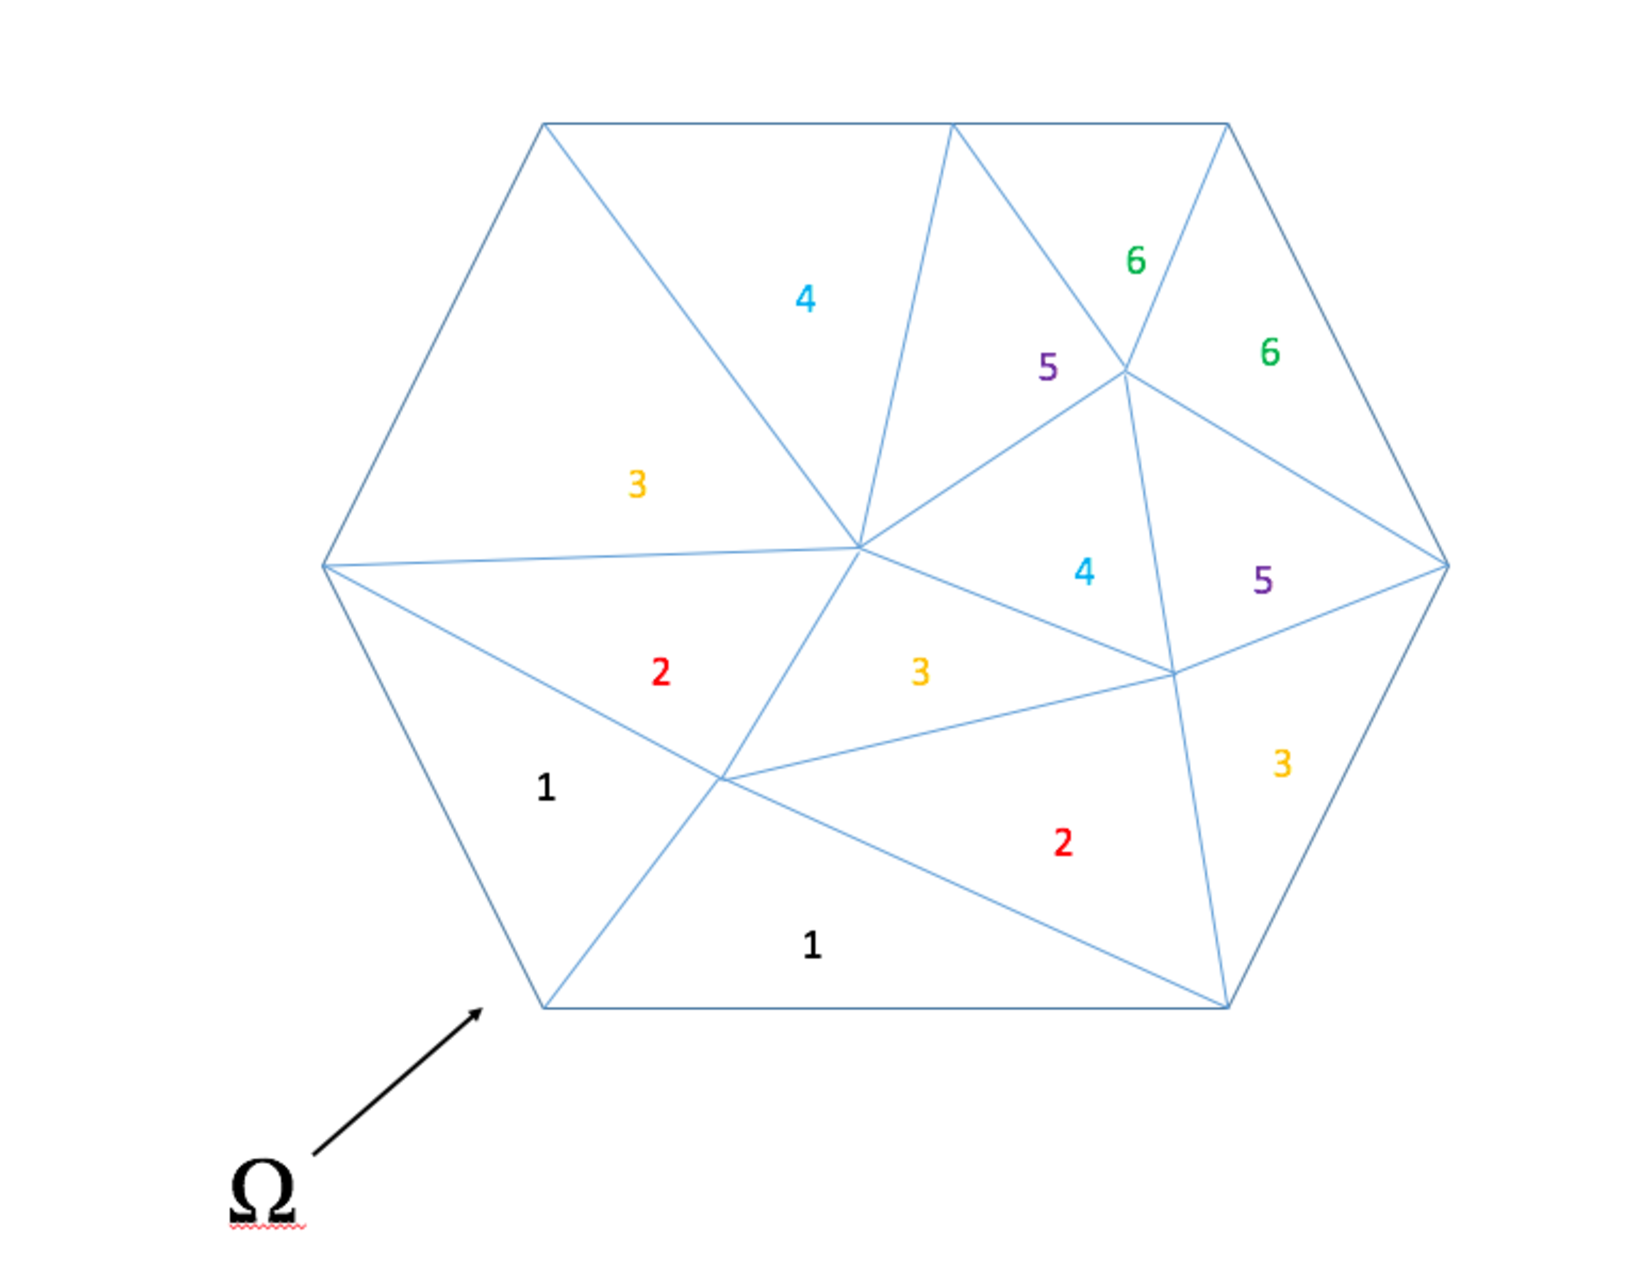
\includegraphics[scale = 0.15]{../figures/UnstructureMesh.pdf}
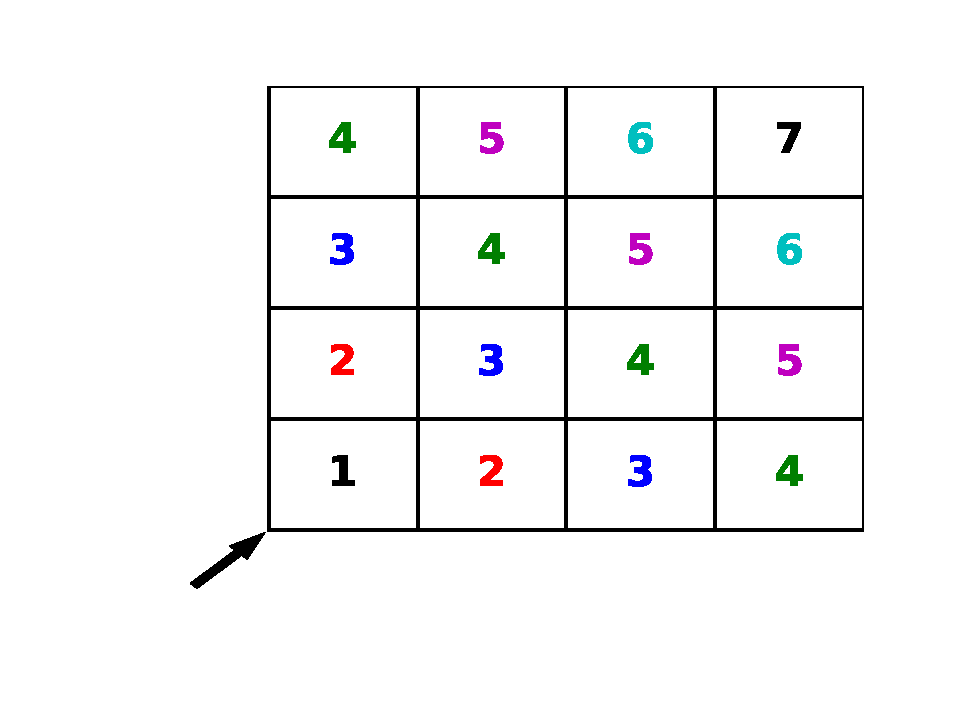
\includegraphics[scale = 0.15]{../figures/StructuredMesh.pdf}
\end{frame}

\begin{frame}[t]\frametitle{Parallel Transport Sweeps}

\begin{block}{A parallel sweep algorithm is defined by three properties:}
\begin{itemize}
\item partitioning: dividing the domain among available processors,
\item aggregation: grouping cells, directions, and energy groups into tasks,
\item scheduling: choosing which task to execute if more than one is available.
\end{itemize}
\end{block}
\end{frame}


\begin{frame}[t]\frametitle{KBA Algorithm}
\begin{block}{}
\begin{itemize}
\item KBA limits the number of processors in $z$ to one, solves one group at a time, and does not aggregate in angle or group.
\item KBA primarily uses a "successive in angle, successive in quadrant" approach.
\item An octant pipelines its angular work, and once all directions are complete, the opposing octant pipelines them back.
\item This is then done for all remaining octant pairs.
\end{itemize}
\end{block}
\end{frame}

\begin{frame}[t]\frametitle{KBA Algorithm}
\begin{block}{}
\begin{itemize}
\item KBA utlilizes a "pipelining" or assembly line approach where new work is started before old work is fully completed.
\end{itemize}
\end{block}
\centering
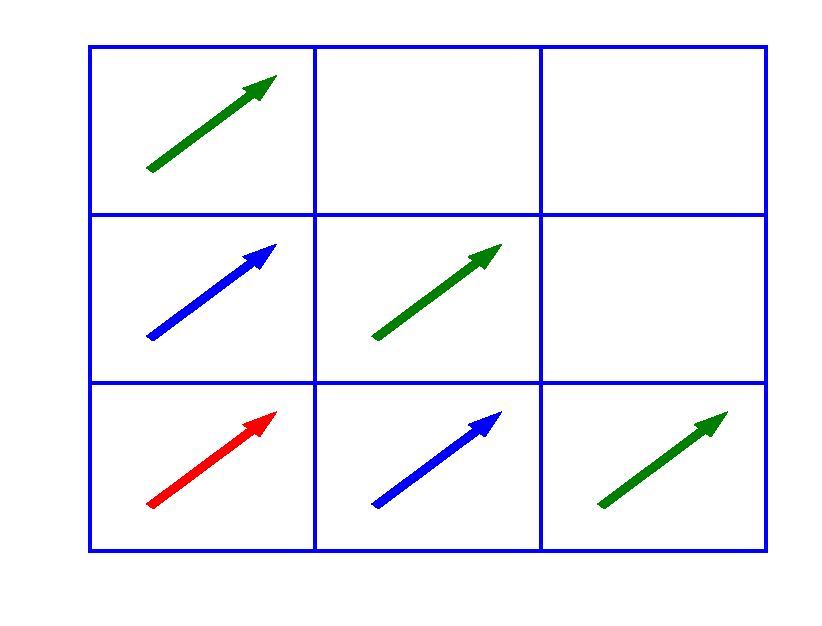
\includegraphics[scale=0.6,trim={0cm 1cm 0cm 0cm},clip]{../figures/pipeline_example.pdf}
\end{frame}

\begin{frame}[t]\frametitle{Sweeps in PDT}
\begin{block}{}
\begin{itemize}
\item PDT's extension of the KBA algorithm does not limit $P_z, A_m, G,$ or $A_g$.
\item PDT also launches all 8 octants (4 quadrants in 2D) simultaneously, rather than one octant-pair at a time.
\item Unlike KBA, PDT must schedule around conflicts that emerge between octants.
\end{itemize}
\end{block}
\end{frame}

\begin{frame}[t]\frametitle{Tie Breaking in PDT}

\begin{block}{If two or more tasks reach a processor at the same time, PDT employs a tie breaking strategy:}

\begin{enumerate}
	\item The task with the greater depth-of-graph remaining (simply, more work remaining) goes first.
	\item If the depth-of-graph remaining is tied, the task with $\Omega_x > 0$ wins.
	\item If multiple tasks have $\Omega_x > 0$, then the task with $\Omega_y > 0$ wins.
	\item If multiple tasks have $\Omega_y > 0$, then the task with $\Omega_z > 0$ wins.
\end{enumerate}
\end{block}
\end{frame}

\begin{frame}[t]\frametitle{Unstructured Meshing in PDT}
  \begin{block}{}
    \begin{itemize}
      \item PDT using unstructured meshes has been a priority since early 2014. 
      \item Unstructured meshes allow for simulation of a wider and more general variety of problems.
      \item Three unstructured mesh types are supported in PDT:
        \begin{itemize}
          \item Triangle (2D and 2D extruded triangular/prismatic meshes).
          \item Spiderweb (2D and 2D extruded prismatic meshes).
          \item Cubit/OpenFOAM (fully unstructured 3D meshes).
        \end{itemize}
    \end{itemize}
  \end{block}
\end{frame}

\begin{frame}[t]\frametitle{Unstructured Meshing in PDT}
\begin{block}{Partitioning for Unstructured Meshes}
\begin{itemize}
\item ``Cut lines" in 2D (cut planes for 3D) are used to slice through the mesh in the $x$, $y$, and $z$ dimensions.
\item The cut planes form brick partitions, called subsets, that have unstructured meshes inside of them. 
\item The subsets are distributed amongst the processor domain.
\end{itemize}
\end{block}
\end{frame}

\begin{frame}[t]\frametitle{Partitioning Example}
\centering
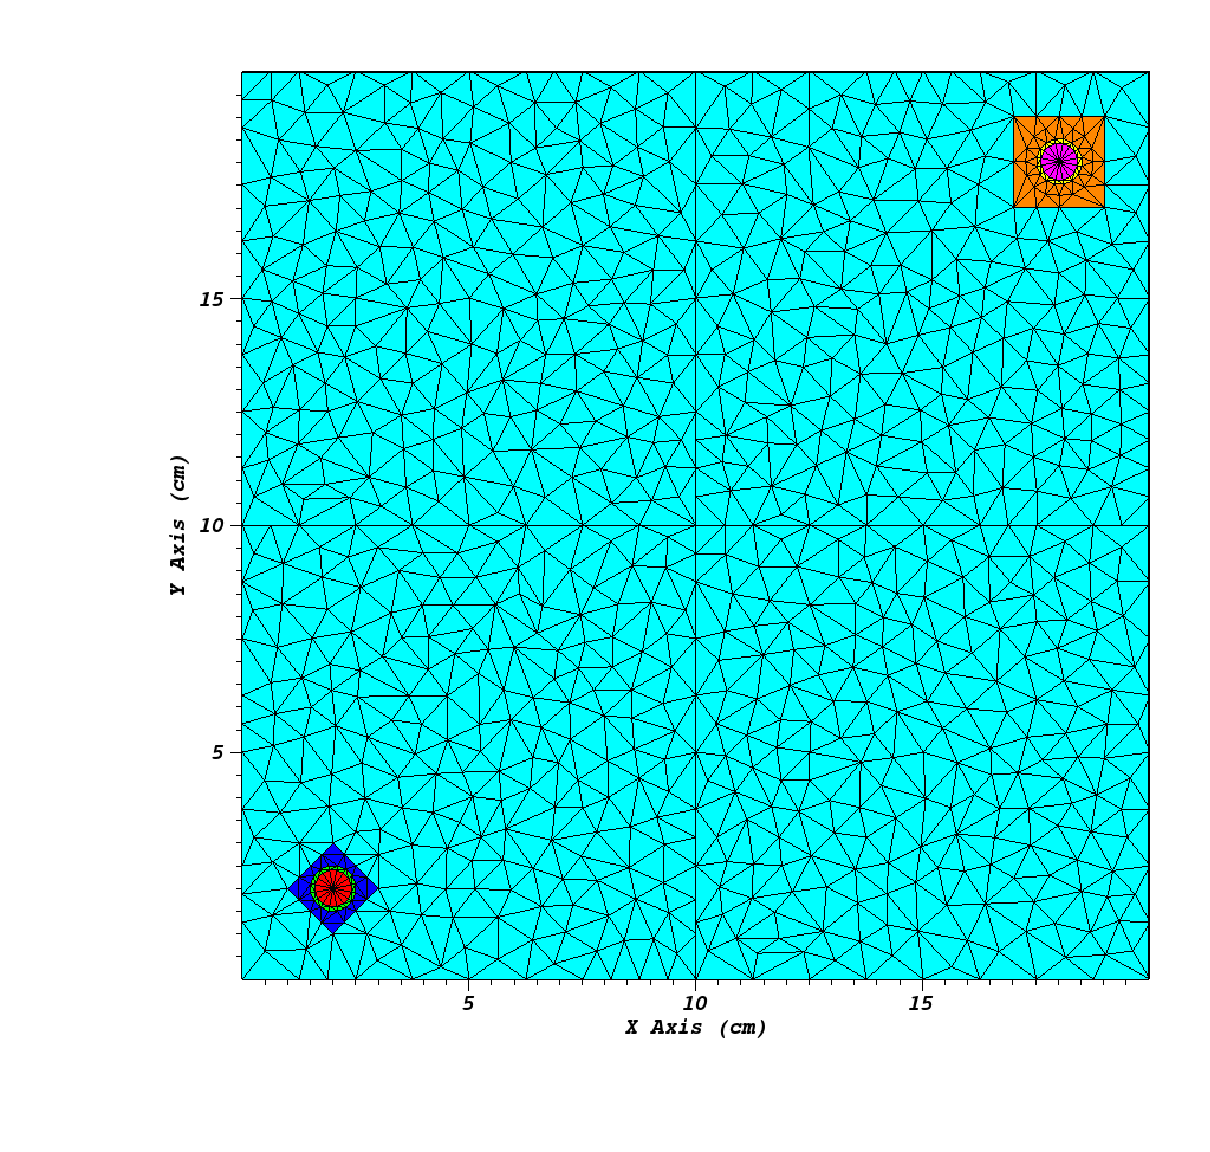
\includegraphics[scale=0.45,trim={0.95in 0.64in 0.35in 0.44in},clip]{../figures/partitioning_example.pdf}
\end{frame}


\section{Load Balancing}
\subsection{}

\begin{frame}[t]\frametitle{Load Balancing}
\begin{block}{Load Balance Metric}
  \begin{itemize}
    \item Max cells per subdomain divided by the average cells per subdomain:
      \begin{itemize}
        \item$f =\frac{\underset{ij}{\text{max}}(N_{ij})}{\frac{N_{tot}}{I\cdot J}}$
      \end{itemize}
    \item Column-wise metric: $f_I = \underset{i}{\text{max}}[\sum_{j} N_{ij}]/\frac{N_{tot}}{I}$
    \item Row-wise metric: $f_J = \underset{j}{\text{max}}[\sum_{i} N_{ij}]/\frac{N_{tot}}{J}$
    \item Per Column row-wise metric: $f_{J_i} = \text{max}[N_{ij}]_i/\frac{\sum_{j}N_{ij}}{J_i}$
  \end{itemize}		
  \tcr{Goal: minimize $f$ using locations of cut lines in X and Y}\\
    
  Subsequent improvement in algorithm: once dimension 1 has been balanced, balance dimension 2, then balance dimension 3 (\tcr{load balancing by dimension})
\end{block}
\end{frame}
\begin{frame}[t]\frametitle{Load Balancing Metrics}
\begin{equation}
f =\frac{\underset{ijk}{\text{max}}(N_{ijk})}{\frac{N_{tot}}{I\cdot J\cdot K}},
\label{metric_def}
\end{equation}
\begin{align}
f_{D1} &= \underset{d1}{\text{max}}[\sum_{d2,d3} N_{ijk}]/\frac{N_{tot}}{D1}, \label{f_d1} \\
f_{D2,d1} &= \Big(\underset{d2}{\text{max}}[\sum_{d3} N_{ijk,d1}]/\frac{N_{d1}}{D2}\Big), \label{f_d2}\\
f_{D3,d2,d1} &= \Big( \underset{d3}{\text{max}}[ N_{ijk,d1,d2}]/\frac{N_{d1,d2}}{D3} \Big) . \label{f_d3}
\end{align}
\end{frame}

\begin{frame}[t]\frametitle{Original Load Balancing Algorithm}
\begin{algorithm}[H]
\label{initial_algorithm}
\begin{algorithmic}

\WHILE{$f > \text{tol}_{\text{subset}}$}
  \IF {$f_I > \text{tol}_{\text{col}}$}
    \STATE Redistribute the X cut planes.
  \ENDIF
  \IF {$f_J > \text{tol}_{\text{row}}$}
  	\STATE Redistribute the Y cut planes.
  \ENDIF
\ENDWHILE
\end{algorithmic}
\end{algorithm}
\end{frame}

\begin{frame}[t]\frametitle{Theoretical Motivation for LBD}
  \begin{block}{}
  \begin{itemize}
    \item Consider simple 2D layout with $M$ unaligned patches of high mesh density
    \item The cellset layout is $[M(N+1)+1] \times [M(N+1)+1]$ but only $MN^2$ cellsets have much work.
    \item Load Imbalance Factor $= \frac{\left( M(N+1)+1 \right)^2}{MN^2} \xrightarrow{N\to \infty} \frac{M^2N^2}{MN^2} = M$
  \end{itemize}
  \end{block}
  \begin{center}
    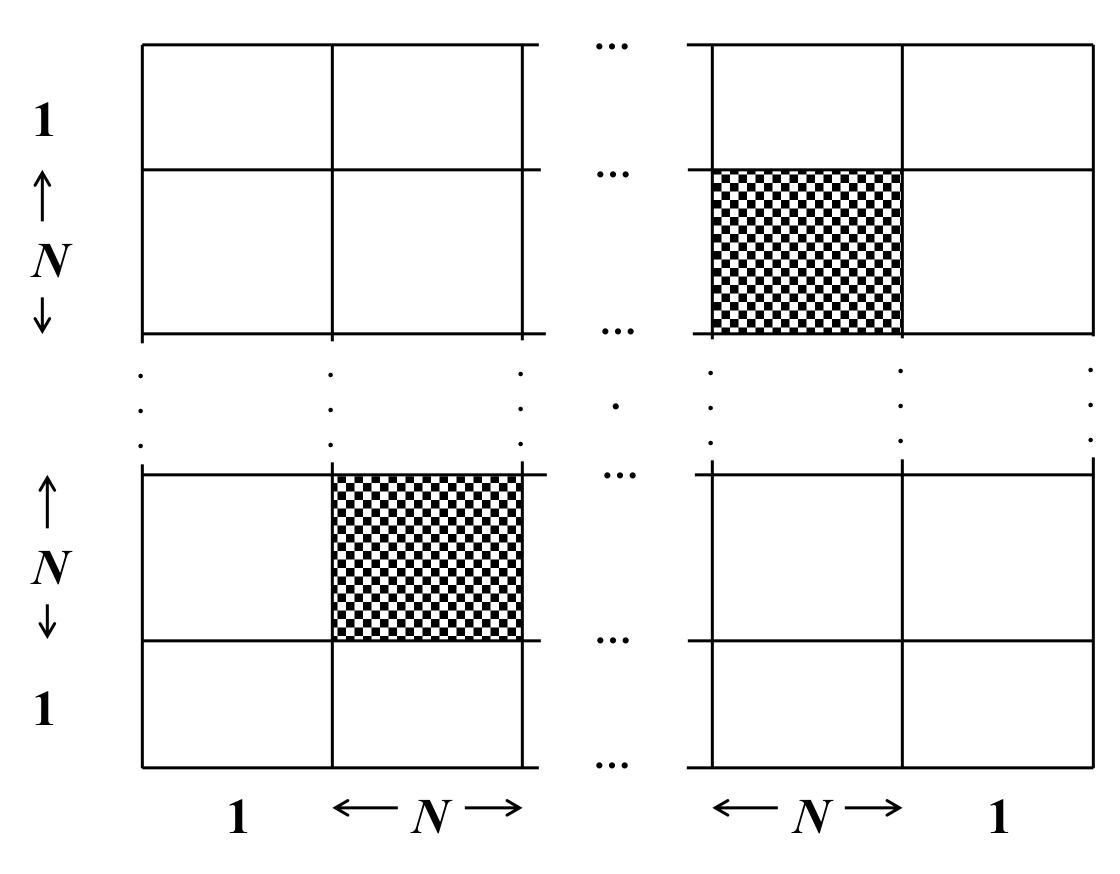
\includegraphics[width=5cm ]{../figures/2dgeneral.png}
  \end{center}
\end{frame}

\begin{frame}[t]\frametitle{Load Balancing By Dimension Algorithm}
\begin{algorithm}[H]
\label{lbd}
\begin{algorithmic}

  \WHILE {$f_{D1} > \text{tol}_{\text{D1}}$}
    \STATE Redistribute the D1 cut planes.
  \ENDWHILE  
  
  \FOR {$d1$ in $D1$}
    \WHILE {$f_{D2,d1} > \text{tol}_{\text{D2}}$}
      \STATE Redistribute the D2 cut planes within d1. 
    \ENDWHILE
  \ENDFOR
  
  \FOR{$d1$ in $D1$}
    \FOR{$d2$ in $D2$}
      \WHILE {$f_{D3,d2,d1} > \text{tol}_{\text{D3}}$ }
        \STATE Redistribute the D3 cut planes within d2 within d1. 
      \ENDWHILE
    \ENDFOR
  \ENDFOR
  
  \STATE Calculate $f$.
\end{algorithmic}
\end{algorithm}
\end{frame}

\begin{frame}[t]\frametitle{Redistribution}
\begin{figure}[H]
\centering
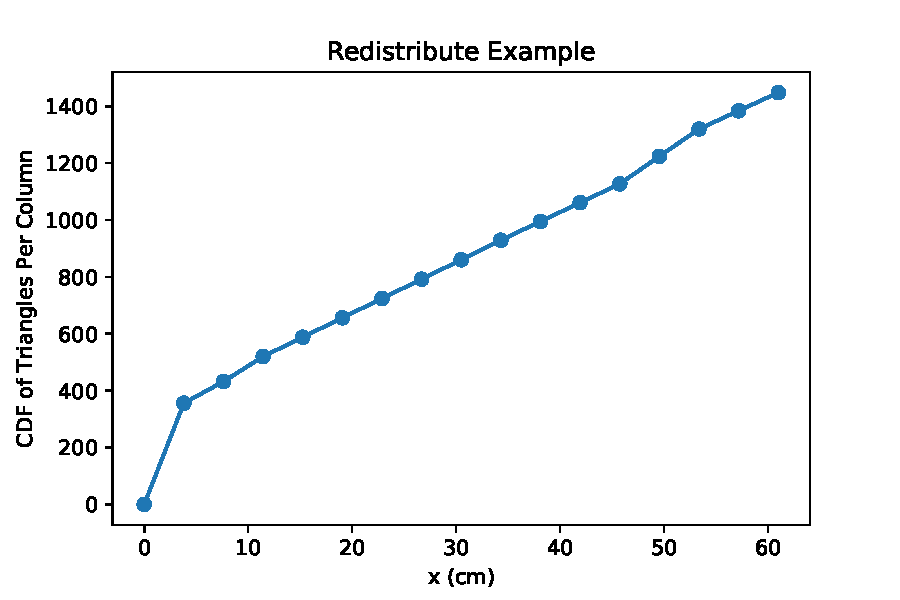
\includegraphics[scale=0.3]{../figures/redistribute_before.pdf}
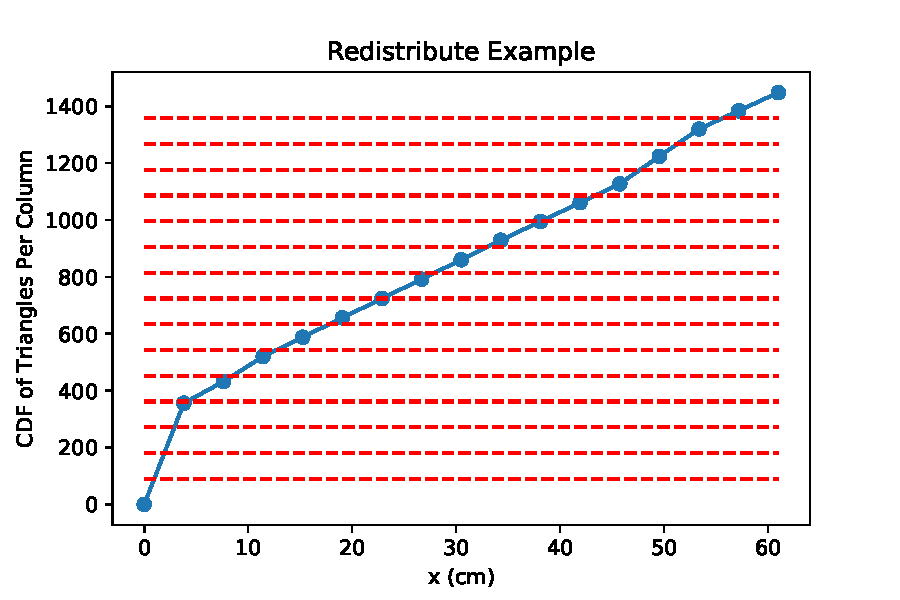
\includegraphics[scale=0.3]{../figures/redistribute_after.pdf}
\caption{The use of the CDF of triangles per column to redistribute the cut planes in X.}
\label{redistribute}
\end{figure}
\end{frame}


\begin{frame}[t]\frametitle{No Load Balancing, f = 41.82}
\centering
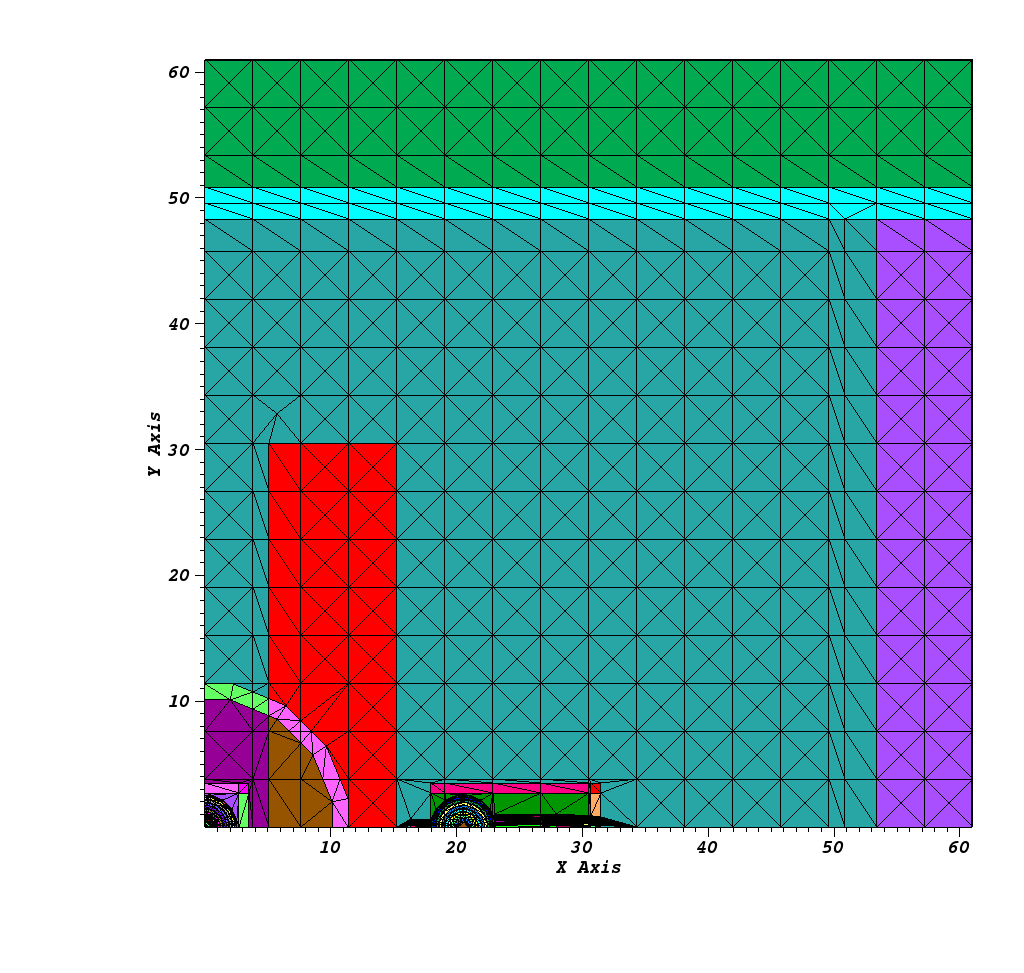
\includegraphics[scale=0.25]{../figures/im12d_nolb.png}
\end{frame}

\begin{frame}[t]\frametitle{Load Balancing, f = 2.97}
\centering
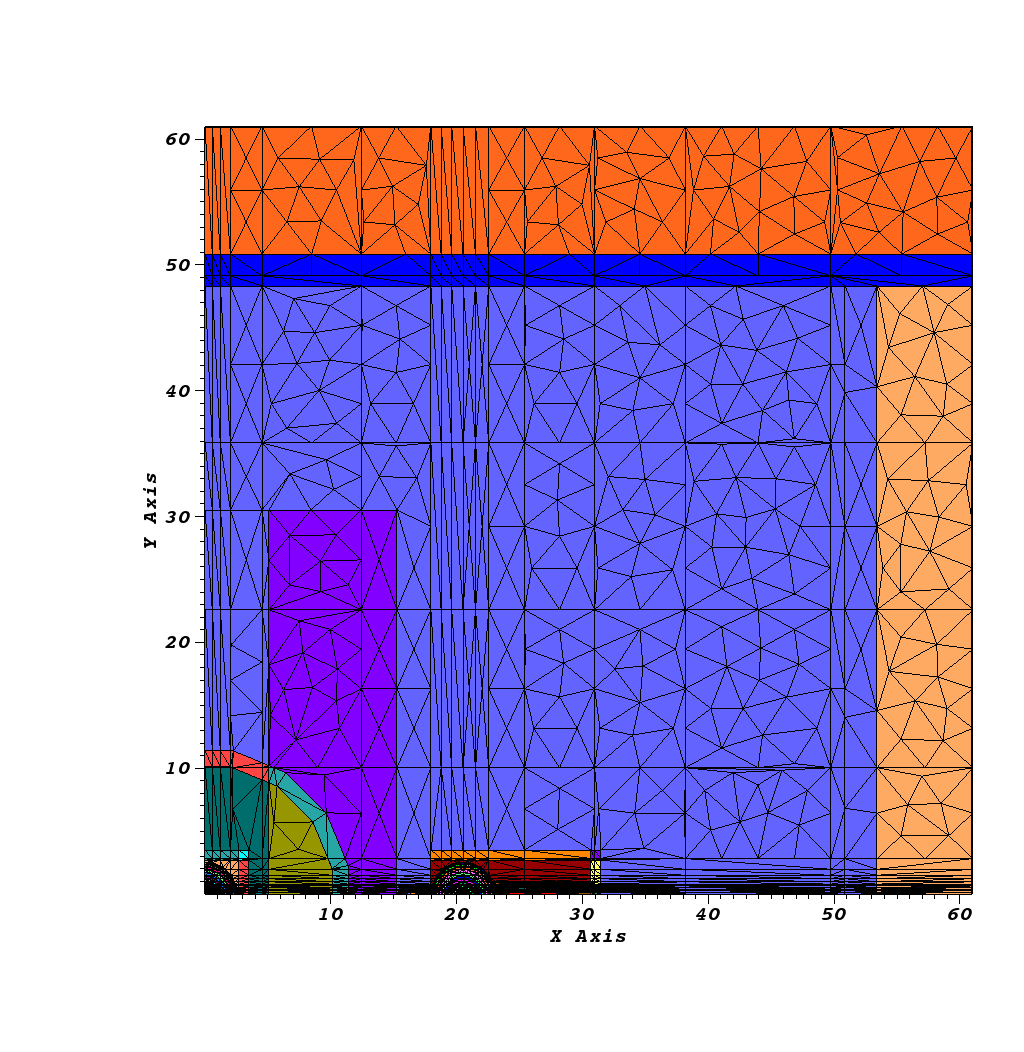
\includegraphics[trim={1cm 0cm 0cm 3cm},clip,scale=0.25]{../figures/im12d_oldlb.png}
\end{frame}


\begin{frame}[t]\frametitle{Load Balancing By Dimension, f = 2.02}
\centering
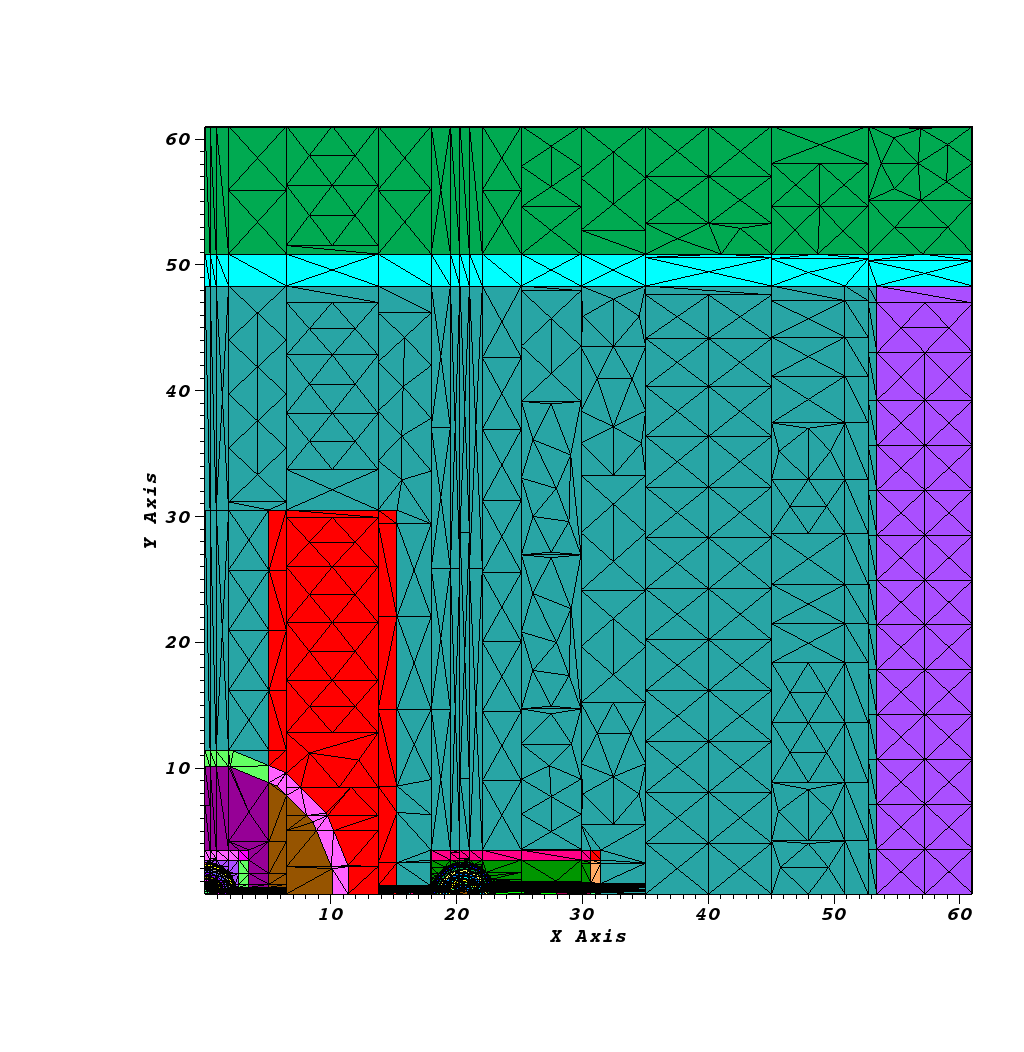
\includegraphics[scale=0.22]{../figures/im12d_newlb.png}
\end{frame}

\begin{frame}[t]\frametitle{3D Load Balancing By Dimension}
\centering
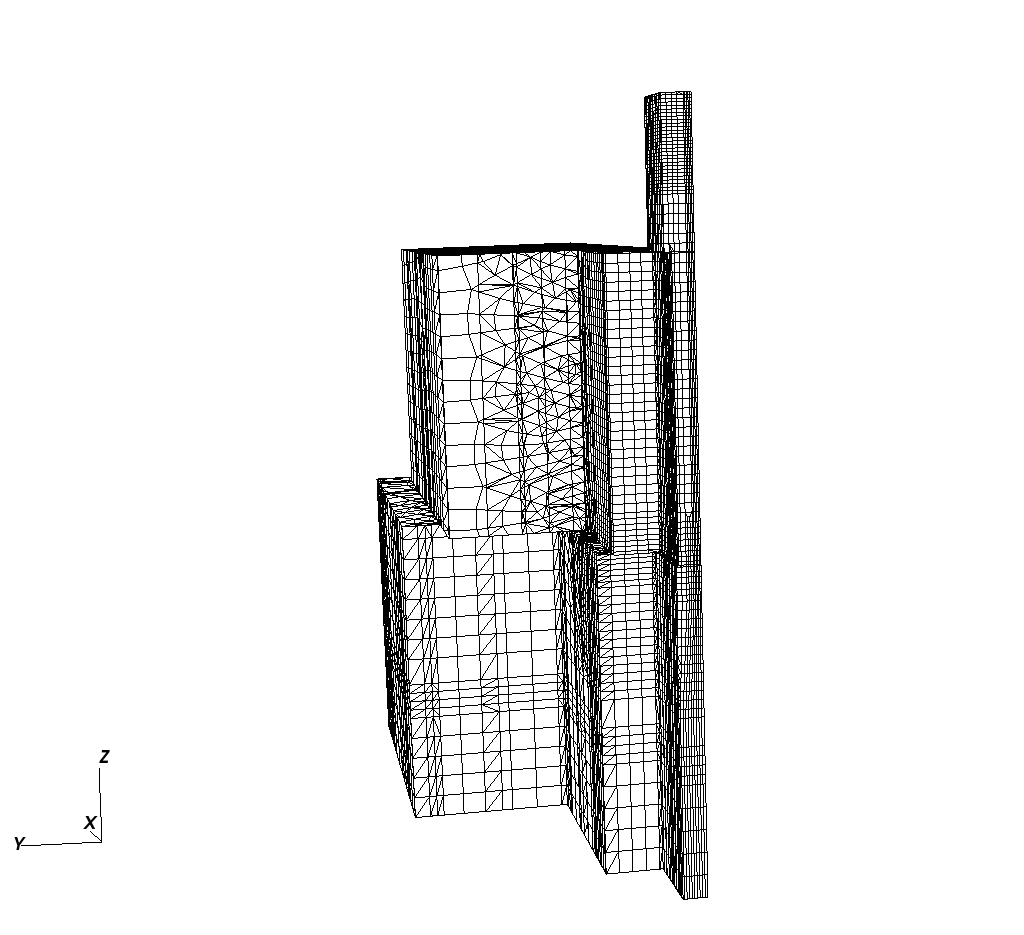
\includegraphics[trim={0cm 1cm 0cm 3cm},clip,scale=0.23]{../figures/im1_foam_448.png}
\end{frame}

\begin{frame}[t]\frametitle{Load Balancing Study}
\begin{figure}[H]
\centering
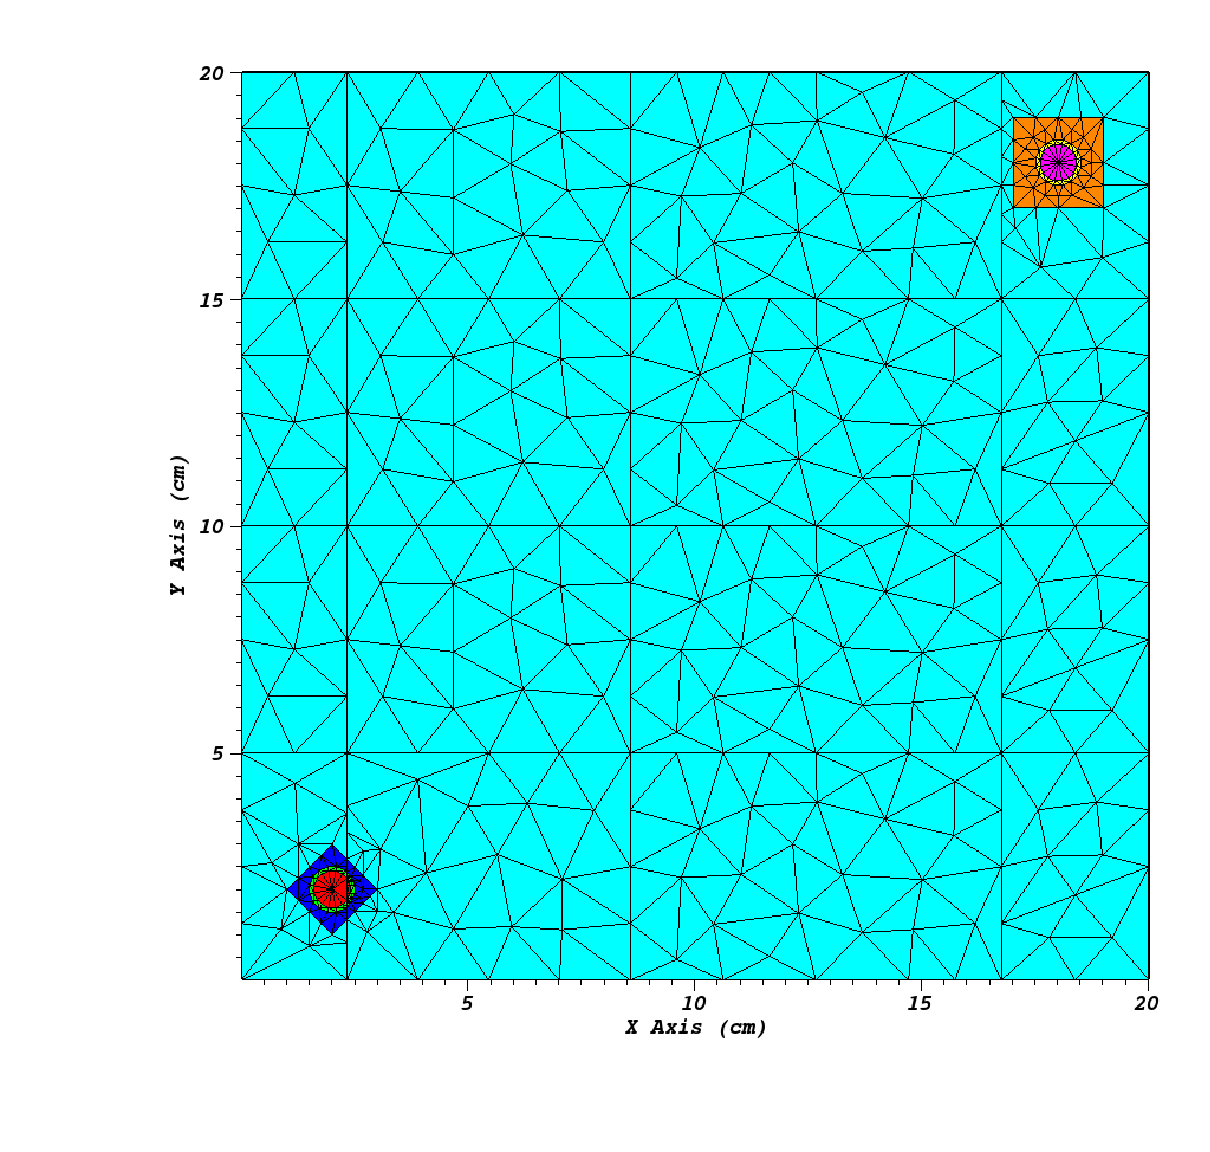
\includegraphics[scale=0.25,trim={0.95in 0.64in 0.35in 0.44in},clip]{../figures/og_lb_example.pdf}
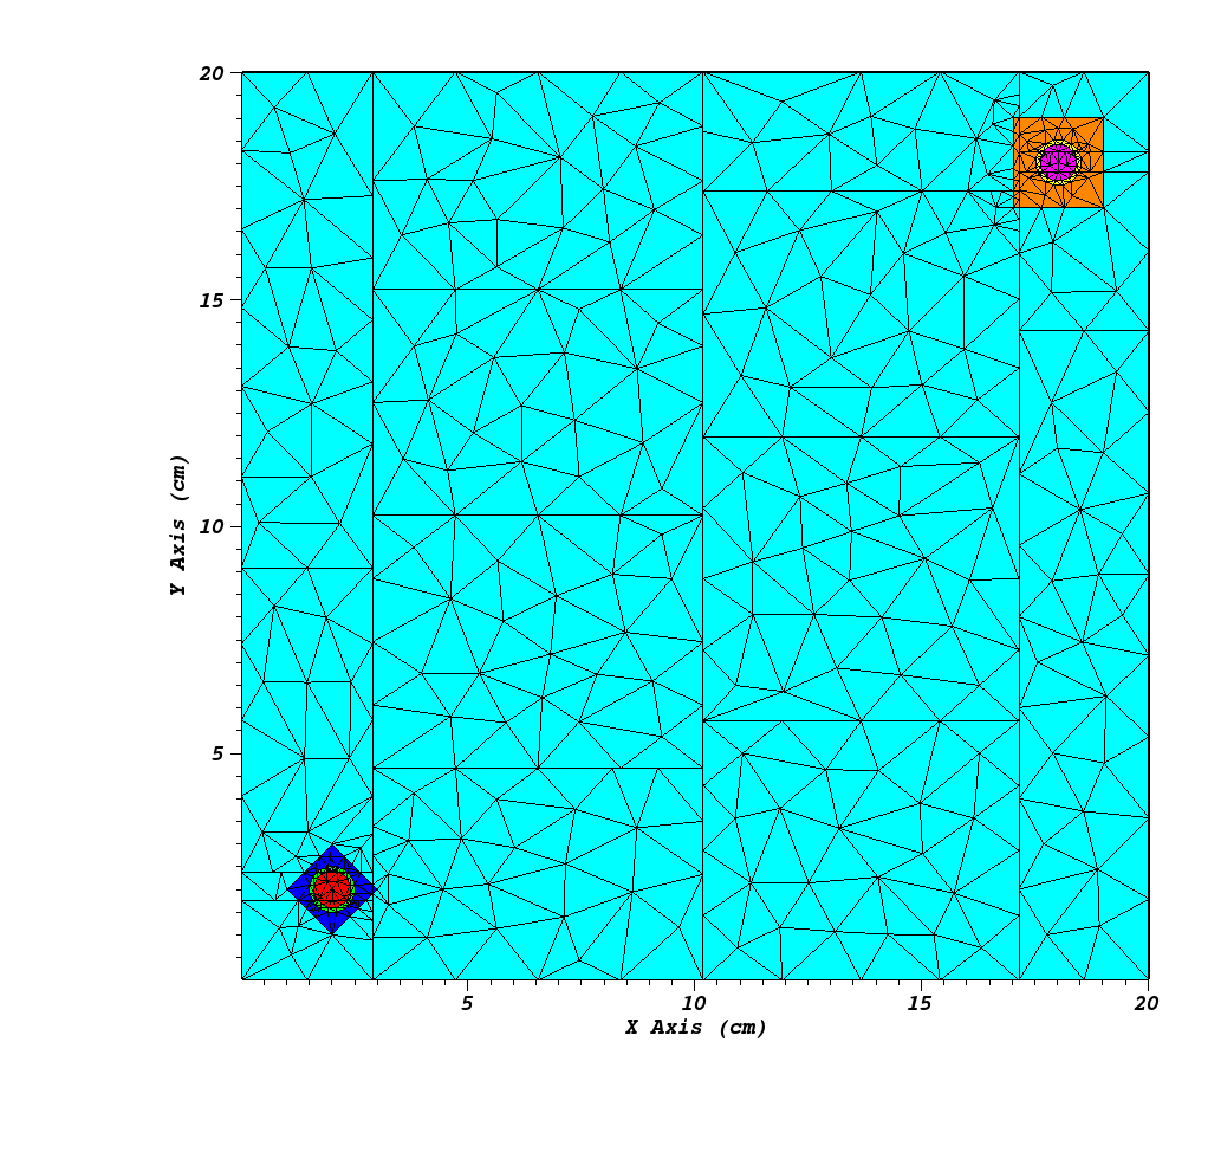
\includegraphics[scale=0.25,trim={0.95in 0.64in 0.35in 0.44in},clip]{../figures/lbd_example.pdf}
\label{alg_illustration}
\end{figure}
  \begin{block}{Parametric Study Parameters}
    \begin{itemize}
      \item Number of subsets ranging from 2 to 10 each in $x$ and $y$.
      \item Maximum triangle area ranging from coarsest possible to 0.01 cm\textsuperscript{2}.
      \item Minimum triangle angle kept constant at $20^{\circ}$.
    \end{itemize}
  \end{block}
\end{frame}

\begin{frame}[t]\frametitle{Load Balancing Study}
\begin{table}[H]
\centering
\caption{\bf The percent improvement of the original load balancing algorithm (left) and the load balancing by dimension algorithm (right).}
\scalebox{0.4}{
\begin{tabular}{c|c|c|c|c|c|c|c|c|c} 

\bf Area, $N^{1/2}$ & \bf  2 & \bf 3    &  \bf  4   &  \bf  5   &  \bf 6    &  \bf  7   &   \bf 8   &  \bf 9    &  \bf 10   \\ \hline \hline
\bf Coarse& 0.000 & 0.367 & 0.403 & 0.552 & 0.628 & 0.491 & 0.890 & 0.720 & 0.765 \\ \hline 
 \bf 1.8& 0.000 & 0.091 & 0.337 & 0.364 & 0.473 & 0.390 & 0.767 & 0.413 & 0.683 \\ \hline 
 \bf 1.6& 0.000 & 0.093 & 0.398 & 0.368 & 0.499 & 0.370 & 0.815 & 0.353 & 0.774 \\ \hline 
 \bf 1.4& 0.000 & 0.061 & 0.080 & 0.410 & 0.415 & 0.412 & 0.570 & 0.413 & 0.545 \\ \hline 
 \bf 1.2& 0.000 & 0.007 & 0.391 & 0.340 & 0.378 & 0.315 & 0.536 & 0.245 & 0.196 \\ \hline 
 \bf 1.0& 0.000 & 0.038 & 0.206 & 0.420 & 0.341 & 0.186 & 0.696 & 0.201 & 0.160 \\ \hline 
 \bf 0.8& 0.000 & 0.049 & 0.109 & 0.336 & 0.434 & 0.139 & 0.637 & 0.228 & 0.000 \\ \hline 
 \bf 0.6& 0.000 & 0.000 & 0.057 & 0.199 & 0.163 & 0.346 & 0.517 & 0.000 & 0.090 \\ \hline 
 \bf 0.4& 0.000 & 0.000 & 0.065 & 0.013 & 0.267 & 0.147 & 0.528 & 0.179 & 0.000 \\ \hline 
 \bf 0.2& 0.000 & 0.000 & 0.000 & 0.000 & 0.001 & 0.041 & 0.566 & 0.121 & 0.000 \\ \hline 
 \bf 0.1& 0.000 & 0.000 & 0.000 & 0.000 & 0.000 & 0.000 & 0.540 & 0.089 & 0.000 \\ \hline 
 \bf 0.08&0.000 & 0.000 & 0.000 & 0.000 & 0.000 & 0.000 & 0.458 & 0.000 & 0.000 \\ \hline 
 \bf 0.06&0.000 & 0.000 & 0.000 & 0.000 & 0.000 & 0.000 & 0.409 & 0.000 & 0.000 \\ \hline 
 \bf 0.05&0.000 & 0.000 & 0.000 & 0.000 & 0.000 & 0.000 & 0.360 & 0.000 & 0.000 \\ \hline 
 \bf 0.04&0.000 & 0.000 & 0.000 & 0.000 & 0.000 & 0.000 & 0.348 & 0.000 & 0.000 \\ \hline 
 \bf 0.03&0.000 & 0.000 & 0.000 & 0.000 & 0.000 & 0.000 & 0.293 & 0.000 & 0.000 \\ \hline 
 \bf 0.02&0.000 & 0.000 & 0.000 & 0.000 & 0.000 & 0.000 & 0.000 & 0.000 & 0.000 \\ \hline 
 \bf 0.01&0.000 & 0.000 & 0.000 & 0.000 & 0.000 & 0.000 & 0.000 & 0.000 & 0.000 \\ \hline 
\end{tabular}}
\scalebox{0.4}{
\begin{tabular}{c|c|c|c|c|c|c|c|c|c} 
\bf Area, $N^{1/2}$ & \bf  2 & \bf 3    &  \bf  4   &  \bf  5   &  \bf 6    &  \bf  7   &   \bf 8   &  \bf 9    &  \bf 10   \\ \hline \hline
\bf Coarse& 0.175 & 0.663 & 0.743 & 0.781 & 0.796 & 0.757 & 0.938 & 0.760 & 0.820 \\ \hline 
  \bf 1.8& 0.266 & 0.417 & 0.511 & 0.661 & 0.766 & 0.665 & 0.896 & 0.647 & 0.512 \\ \hline 
  \bf 1.6& 0.262 & 0.426 & 0.568 & 0.635 & 0.760 & 0.631 & 0.897 & 0.542 & 0.557 \\ \hline 
  \bf 1.4& 0.244 & 0.369 & 0.497 & 0.618 & 0.769 & 0.595 & 0.901 & 0.722 & 0.741 \\ \hline 
  \bf 1.2& 0.242 & 0.336 & 0.552 & 0.614 & 0.663 & 0.583 & 0.886 & 0.208 & 0.597 \\ \hline 
  \bf 1.0& 0.203 & 0.287 & 0.458 & 0.549 & 0.442 & 0.605 & 0.875 & 0.536 & 0.552 \\ \hline 
  \bf 0.8& 0.162 & 0.330 & 0.435 & 0.460 & 0.638 & 0.542 & 0.888 & 0.393 & 0.000 \\ \hline 
  \bf 0.6& 0.122 & 0.291 & 0.447 & 0.460 & 0.503 & 0.610 & 0.844 & 0.267 & 0.058 \\ \hline 
  \bf 0.4& 0.093 & 0.274 & 0.310 & 0.400 & 0.488 & 0.519 & 0.888 & 0.328 & 0.000 \\ \hline 
  \bf 0.2& 0.042 & 0.147 & 0.185 & 0.267 & 0.344 & 0.299 & 0.810 & 0.349 & 0.025 \\ \hline 
  \bf 0.1& 0.026 & 0.067 & 0.109 & 0.156 & 0.144 & 0.210 & 0.735 & 0.367 & 0.000 \\ \hline 
  \bf 0.08&0.002 & 0.032 & 0.059 & 0.060 & 0.122 & 0.150 & 0.699 & 0.268 & 0.041 \\ \hline 
  \bf 0.06&0.005 & 0.014 & 0.036 & 0.057 & 0.094 & 0.073 & 0.643 & 0.246 & 0.058 \\ \hline 
  \bf 0.05&0.006 & 0.017 & 0.006 & 0.005 & 0.033 & 0.068 & 0.579 & 0.208 & 0.008 \\ \hline 
  \bf 0.04&0.002 & 0.008 & 0.009 & 0.000 & 0.011 & 0.022 & 0.544 & 0.168 & 0.000 \\ \hline 
  \bf 0.03&0.002 & 0.000 & 0.005 & 0.024 & 0.028 & 0.027 & 0.479 & 0.089 & 0.000 \\ \hline 
  \bf 0.02&0.003 & 0.002 & 0.001 & 0.000 & 0.001 & 0.004 & 0.361 & 0.070 & 0.000 \\ \hline 
  \bf 0.01&0.002 & 0.003 & 0.002 & 0.000 & 0.001 & 0.000 & 0.196 & 0.027 & 0.000 \\ \hline 

\end{tabular}}
\label{all_improvements}
\end{table}
\end{frame}

\begin{frame}[t]\frametitle{Paramtric Study Conclusions}
  \begin{block}{}
  \begin{itemize}
    \item The more uniformly refined your mesh, the more inherently balanced it is.
    \item With the exception of a few outliers, the load balancing by dimension algorithm was an improvement over the original load balancing algorithm.
    \item The metric improved by a max of 76.9\% and a mean of 21.7\% with the load balancing by dimension algorithm over the original load balancing algorithm. 
  \end{itemize}
  \end{block}
\end{frame}

\begin{frame}[t]\frametitle{Consequences of Load Balancing By Dimension}
  \begin{block}{}
  \begin{itemize}
    \item Perfect load balance in some cases will come at the cost of optimal sweeping.
    \item Time to solution is the most important parameter, and if keeping a more optimal sweeping grid means a less balanced problem, then so be it.
    \item The concept of a stage may be misleading when dealing with imbalanced partitions, as we cannot easily characterize the idle time.
    \item A time-to-solution estimator must be built to more accurately predict sweep time.
  \end{itemize}
  \end{block}
\end{frame}

\begin{frame}[t]\frametitle{Sweep on Regular Grid with 3 Angle Sets}
    \centering
	\animategraphics[loop,controls,width=0.7\linewidth]{10}{../figures/sweeps_png/sweep_regular_20x20_as3_dog/sweep_regular_20x20_as3_dog_}{1}{48}
	%\href{run:figures/sweep_figs/sweeps_png/sweep_regular_20x20_as3_dog/animation.gif}{Animation.gif}
\end{frame}

\begin{frame}[t]\frametitle{Sweep on LBD Grid with 3 Angle Sets}
   \centering
	\animategraphics[loop,controls,width=0.7\linewidth]{10}{../figures/sweeps_png/sweep_random_20x20_as3_dog/sweep_random_20x20_as3_dog_}{1}{101}
	%\href{run:figures/sweep_figs/sweeps_png/sweep_random_20x20_as3_dog/animation.gif}{Animation.gif}
\end{frame}


\begin{frame}[t]\frametitle{Sweep on Worst Grid with 1 Angle Set}
    \centering
	\animategraphics[loop,controls,width=0.7\linewidth]{10}{../figures/sweeps_png/sweep_worst_20x20_as1_dog/sweep_worst_20x20_as1_dog_}{1}{230}
	%\href{run:figures/sweep_figs/sweeps_png/sweep_worst_20x20_as1_dog/animation.gif}{Animation.gif}
\end{frame}

%%%%%%%%%%%%%%%%%%%%%%%%%%%%%%%%%%%%%%%%%%%%%%%%%%%%%%%%%%%%%%%%%%%%%%%%%%%%%%%%%%%%%%%
%%%%%%%%%%%%%%%%%%%%%%%%%%%%%%%%%%%%%%%%%%%%%%%%%%%%%%%%%%%%%%%%%%%%%%%%%%%%%%%%%%%%%%%
%%%%%%%%%%%%%%%%%%%%%%%%%%%%%%%%%%%%%%%%%%%%%%%%%%%%%%%%%%%%%%%%%%%%%%%%%%%%%%%%%%%%%%%
\section{Time-To-Solution Estimator}
\subsection{}
%%%%%%%%%%%%%%%%%%%%%%%%%%%%%%%%%%%%%%%%%%%%%%%%%%%%%%%%%%%%%%%%%%%%%%%%%%%%%%%%%%%%%%%
%%%%%%%%%%%%%%%%%%%%%%%%%%%%%%%%%%%%%%%%%%%%%%%%%%%%%%%%%%%%%%%%%%%%%%%%%%%%%%%%%%%%%%%
%%%%%%%%%%%%%%%%%%%%%%%%%%%%%%%%%%%%%%%%%%%%%%%%%%%%%%%%%%%%%%%%%%%%%%%%%%%%%%%%%%%%%%%

\begin{frame}[t]\frametitle{Overview}
\begin{block}{}
\begin{itemize}
	\item We need to optimize the cut line location not for balance, but for the best possible sweep time.
	\item We must build a time-to-solution estimator that calculates the time to solution for a given cut line partitioning.
	\item The time to solution estimator will be fed into an optimizing function that minimizes the time to solution. The cut lines corresponding to the minimum time to solution are the optimal partitioning scheme.
\end{itemize}
\end{block}
\begin{block}{IMPORTANT}
The time-to-solution estimator is a graph-based method that uses graph algorithms that rely on an acyclic graph. The partitioning schemes used CANNOT induce cycles.
\end{block}
\end{frame}

\begin{frame}[t]\frametitle{Time To Solution Estimator}
\begin{block}{}
\begin{enumerate}
    \item Given a partitioning scheme, build an adjacency matrix.
    \item From the adjacency matrix, build Directed Acyclic Graphs (DAGs), one for each quadrant/octant.
    \item Weight each DAG's edges based on the solve and communication time of each subset to its neighbors.
    \item Adjust the weights of each graph to reflect a universal timescale.
    \item Adjust the weights of each graph based on the number of anglesets.
    \item Adjust the weights of each graph to reflect sweep conflicts between octants.
    \item Obtain the time-to-solution.
\end{enumerate}
\end{block}
\end{frame}

\begin{frame}[t]\frametitle{Building the Adjacency Matrix}
\begin{block}{}
\begin{itemize}
  \item The adjacency matrix provides the crucial connectivity information necessary to build the Task Dependence Graphs (TDG's) in the time-to-solution estimator.
\end{itemize}
\end{block}
\begin{minipage}{0.49\textwidth}
\centering
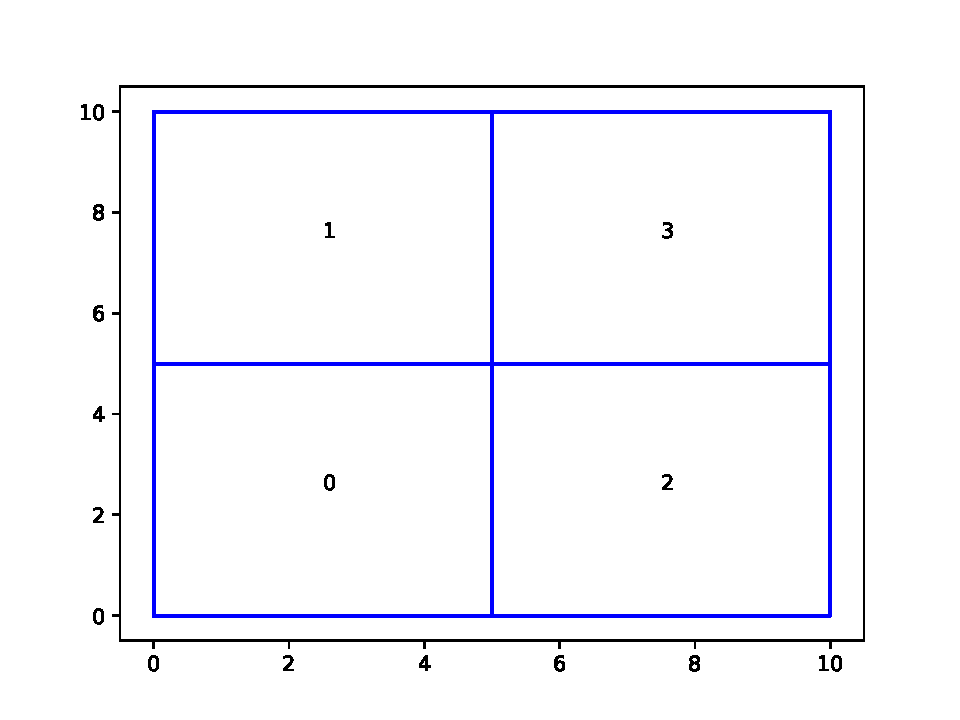
\includegraphics[scale=0.4]{../figures/base_adjacency_layout.pdf}
\end{minipage}
\begin{minipage}{0.49\textwidth}
\centering
$\begin{pmatrix}
0 & 1 & 1  & 0  \\
1 & 0 & 0 & 1 \\
1 & 0 & 0 & 1 \\ 
0 & 1 & 1 & 0 \\
\end{pmatrix}$
\end{minipage}
\end{frame}

\begin{frame}[t]\frametitle{Building the Task Dependence Graphs}
\begin{block}{}
\begin{itemize}
    \item Each quadrant/octant gets its own TDG.
    \item The opposing quadrant/octant pairs have opposing sweep orderings. 
    \item Each set of quadrant/octant pairs uses a different adjacency matrix. 
    \item Python package \textbf{networkx} is used for all graph operations.
\end{itemize}
\end{block}
\centering
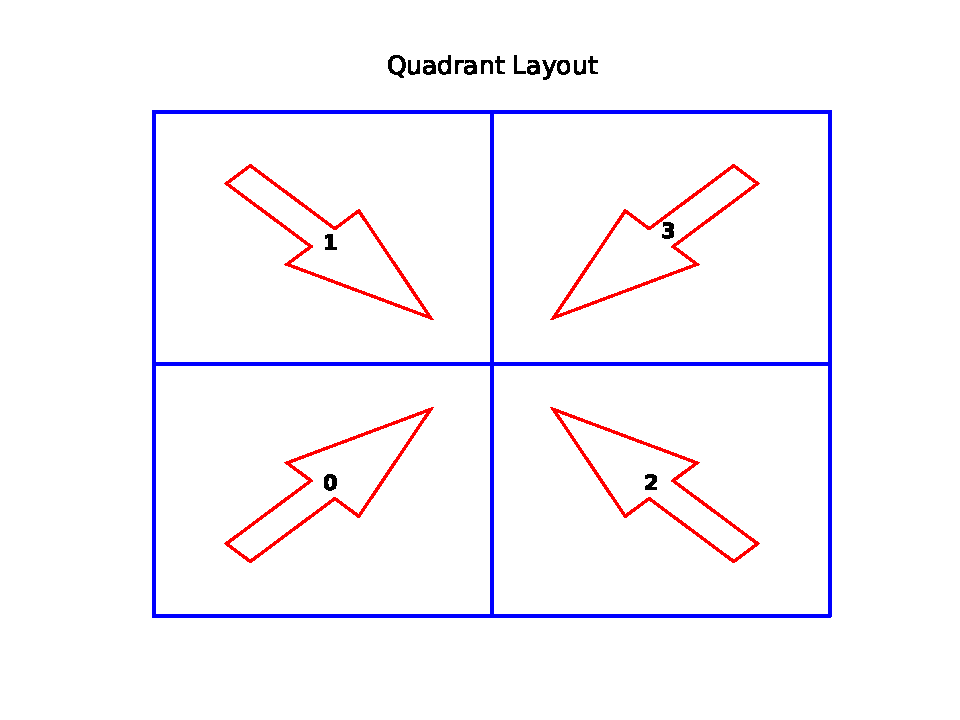
\includegraphics[scale=0.45]{../figures/quadrant_layout.pdf}
\end{frame}

\begin{frame}[t]\frametitle{Quadrants 0 and 3}
\begin{block}{}
\begin{itemize}
    \item We use the upper triangular portion of the adjacency matrix for quadrant 0.
    \item We use the lower triangular portion of the adjacency matrix for quadrant 1.
\end{itemize}
\end{block}
\begin{minipage}{0.49\textwidth}
  \centering
  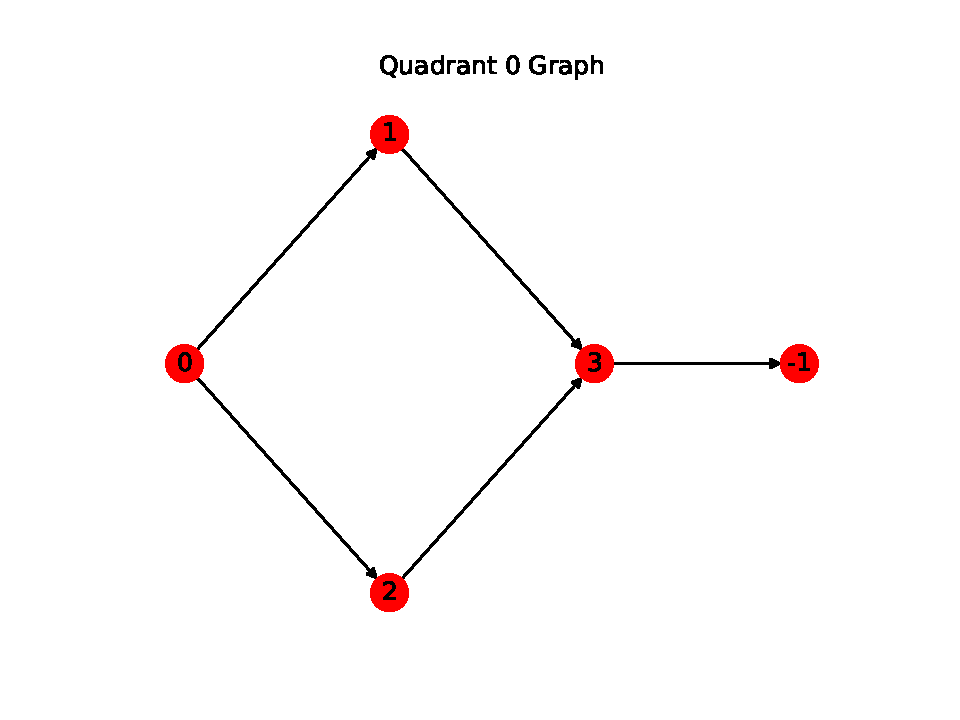
\includegraphics[scale=0.35]{../figures/q0_preweight.pdf}
\end{minipage}
\begin{minipage}{0.49\textwidth}
  \centering
  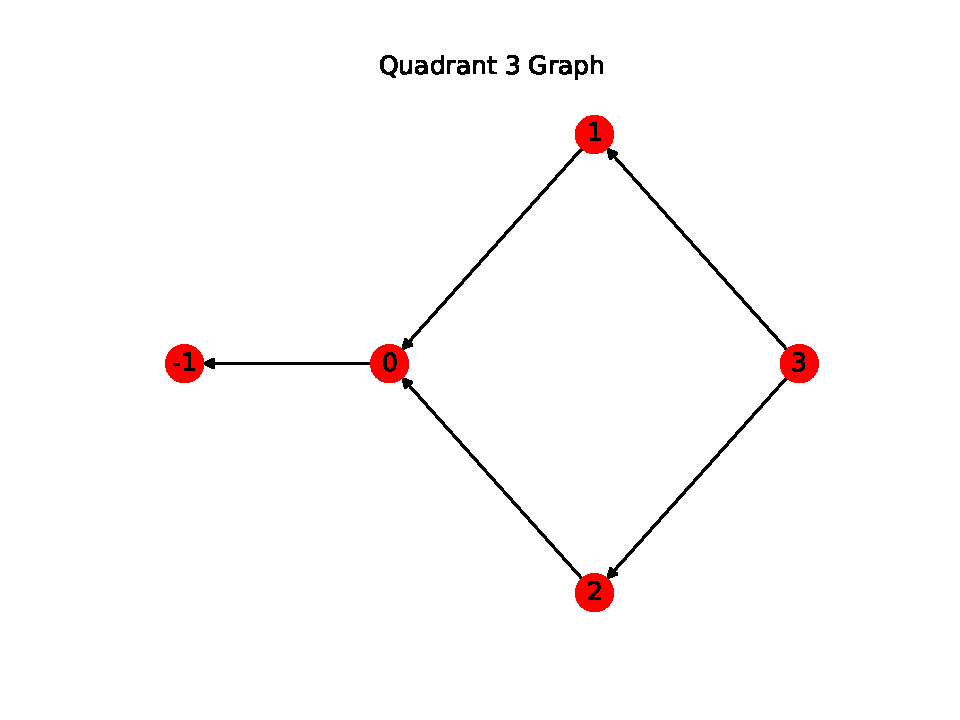
\includegraphics[scale=0.35]{../figures/q3_preweight.pdf}
\end{minipage}
\end{frame}

\begin{frame}[t]\frametitle{Quadrants 1 and 2}
  \begin{block}{}
    \begin{itemize}
      \item Before building the graphs for these opposing quadrants, we have to alter the adjacency matrix slightly.
      \item The subsets get renumbered in a manner where subset 1 becomes subset 0, subset 0 becomes subset 1, etc. In short the column numbering is flipped, and a ``flipped'' adjacency matrix is built. 
    \end{itemize}
  \end{block}
  \begin{minipage}{0.49\textwidth}
    \centering
    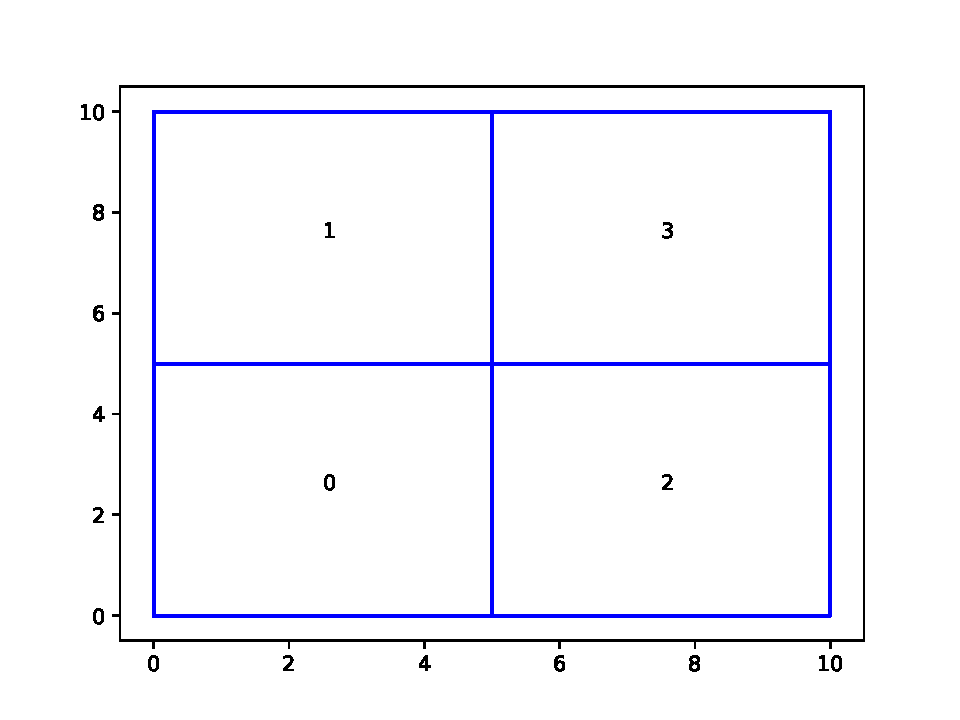
\includegraphics[scale=0.38]{../figures/base_adjacency_layout.pdf}
  \end{minipage}
  \begin{minipage}{0.49\textwidth}
    \centering
    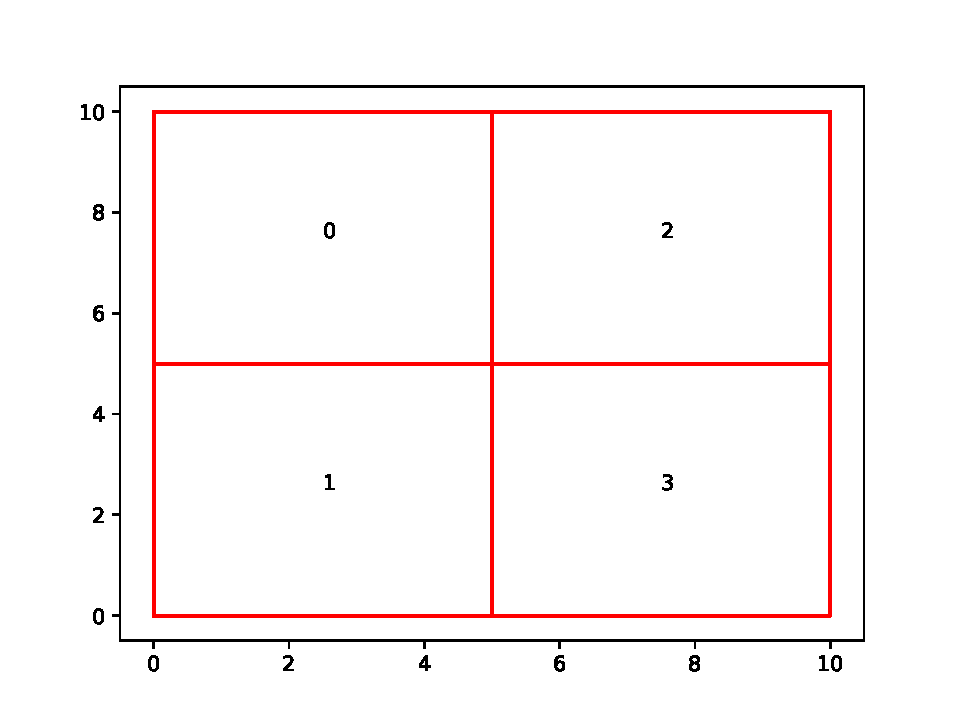
\includegraphics[scale=0.38]{../figures/flipped_subset_layout.pdf}
  \end{minipage}
\end{frame}

\begin{frame}[t]\frametitle{Quadrants 1 and 2}
  \begin{block}{}
    \begin{itemize}
      \item We use the upper triangular portion of the ``flipped'' adjacency matrix for quadrant 1.
      \item We use the lower triangular portion of the ``flipped'' adjacency matrix for quadrant 2.
    \end{itemize}
  \end{block}
  \begin{minipage}{0.49\textwidth}
    \centering
    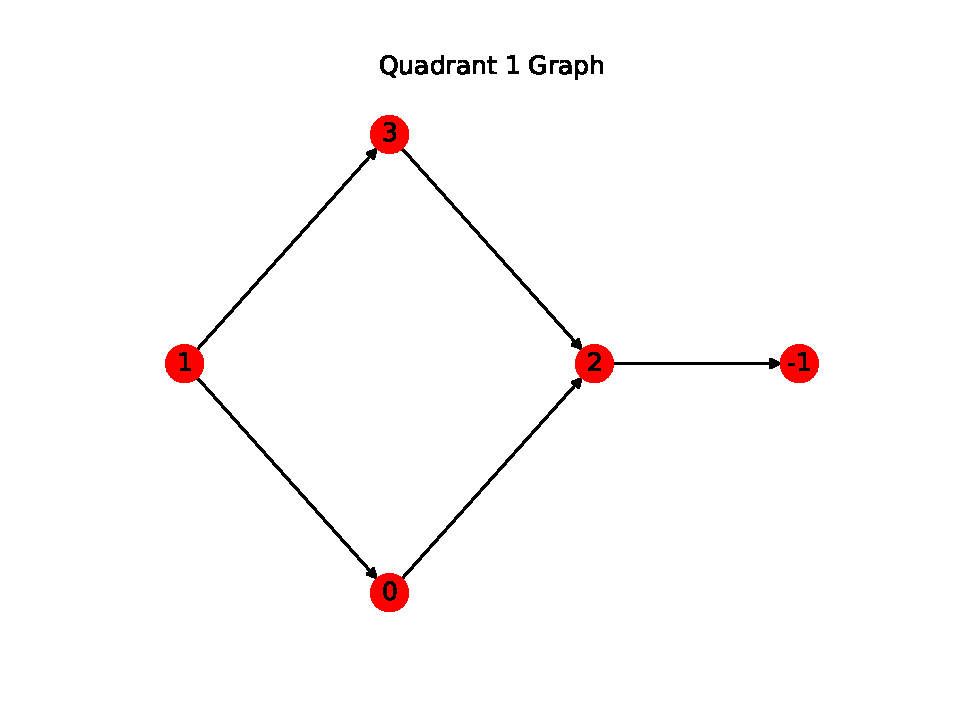
\includegraphics[scale=0.35]{../figures/q1_preweight.pdf}
  \end{minipage}
  \begin{minipage}{0.49\textwidth}
    \centering
    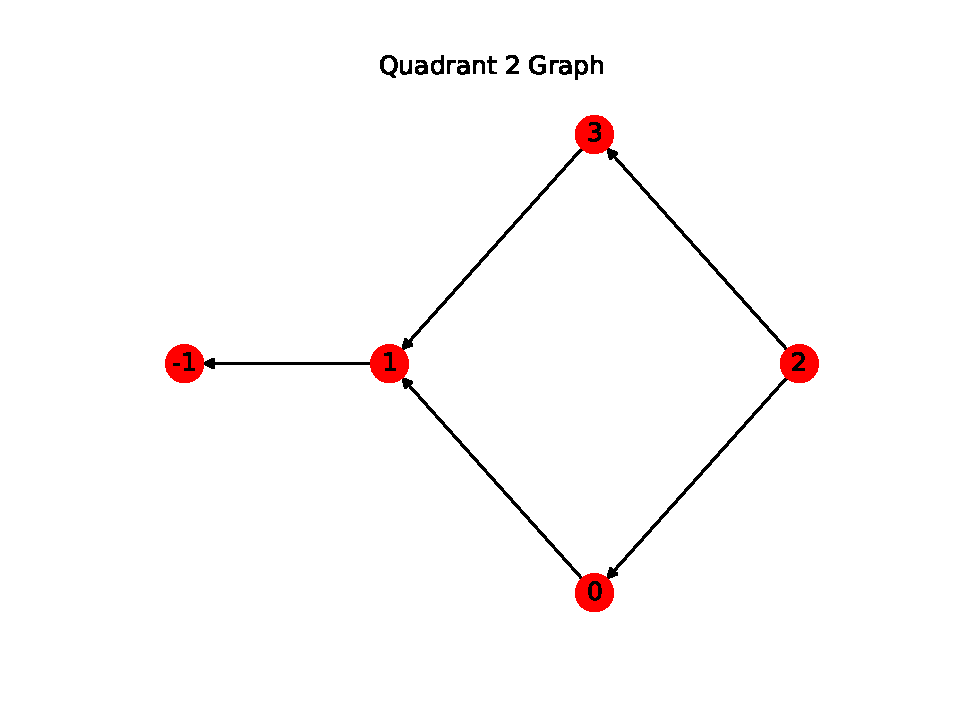
\includegraphics[scale=0.35]{../figures/q2_preweight.pdf}
  \end{minipage}
\end{frame}

\begin{frame}[t]\frametitle{Weighting the TDGs}
  \begin{block}{}
    \begin{itemize}
    	\item In order to weight the graph properly, we need to have a mesh density function that we can calculate the cells (and then unknowns) per subset from.
    	\item The weight of the edge between two nodes (subsets) in the graph represents the solve and communication time of the base node.
    \end{itemize}
  \end{block}
  \begin{block}{}
    \begin{align}
    \text{cells per subset} &= \int_{\tcr{x_i}}^{\tcr{x_{i+1}}} \int_{\tcr{y_j}}^{\tcr{y_{j+1}}} \int_{\tcr{z_k}}^{\tcr{z_{k+1}}} \text{mesh density } dx dy dz \\
    \label{weight}
    \text{weight} &= N_u\cdot T_u + N_b\cdot T_{\text{comm}} + \text{latency}\cdot M_L \\
    N_u &= \text{num cells}\cdot \text{unknowns per cell} \\
    N_b &\approx(\text{num boundary cells})\cdot \text{boundary unknowns per cell}
    \end{align}
  \end{block}
\end{frame}

\begin{frame}[t]\frametitle{Weighting the TDGs}
  \begin{minipage}{0.49\textwidth}
    \centering
    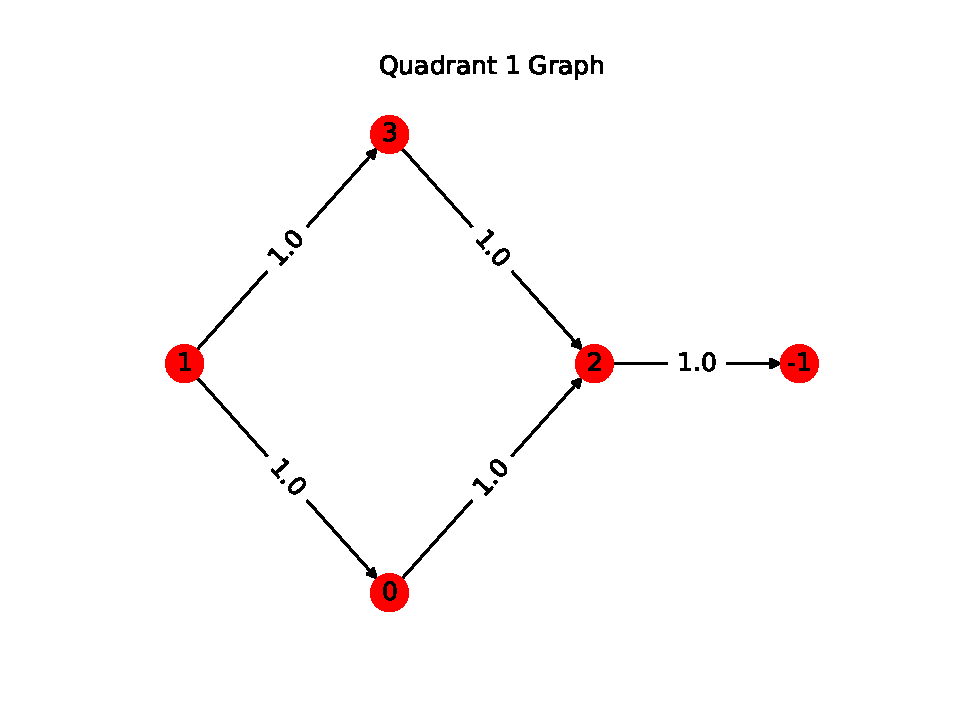
\includegraphics[scale=0.32]{../figures/q1_postweight.pdf}
  \end{minipage}
  \begin{minipage}{0.49\textwidth}
    \centering
    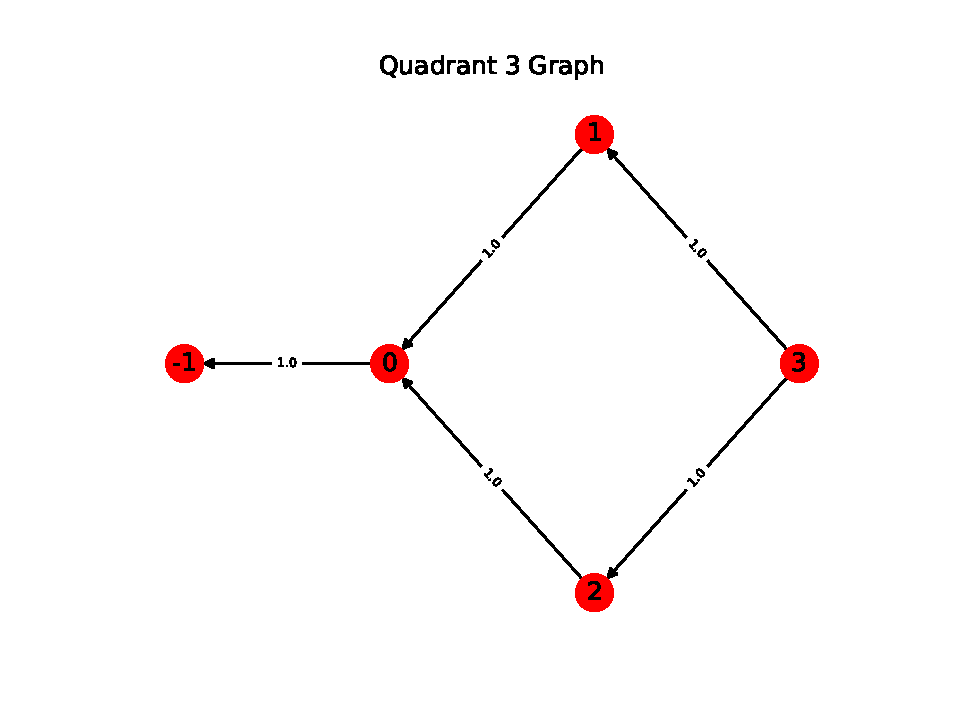
\includegraphics[scale=0.32]{../figures/q3_postweight.pdf}
  \end{minipage}
  \begin{minipage}{0.49\textwidth}
    \centering
    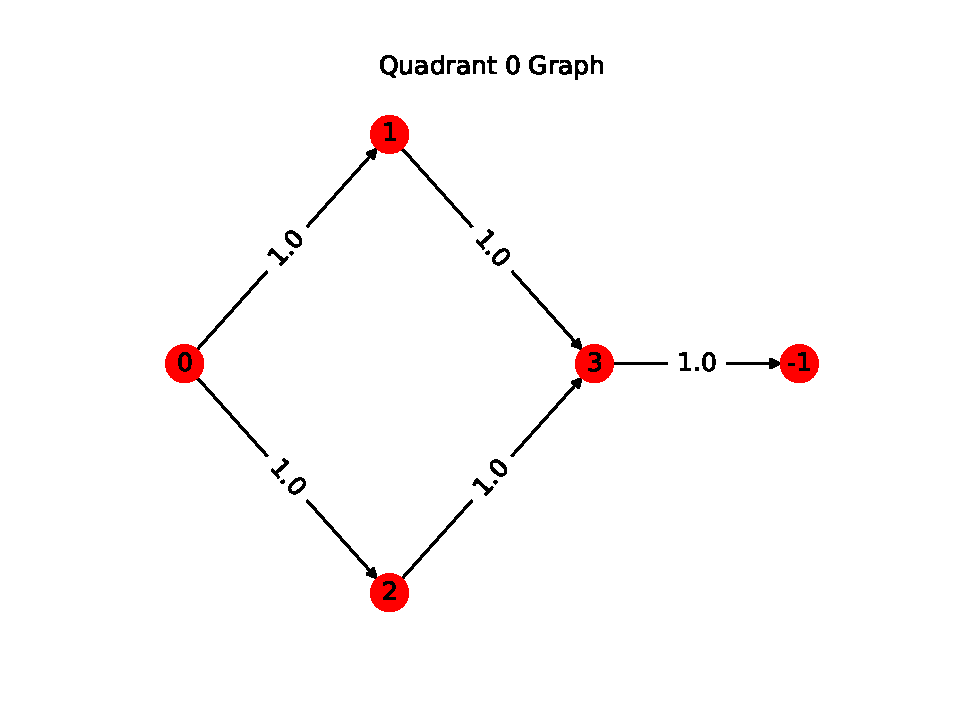
\includegraphics[scale=0.32]{../figures/q0_postweight.pdf}
  \end{minipage}
  \begin{minipage}{0.49\textwidth}
    \centering
    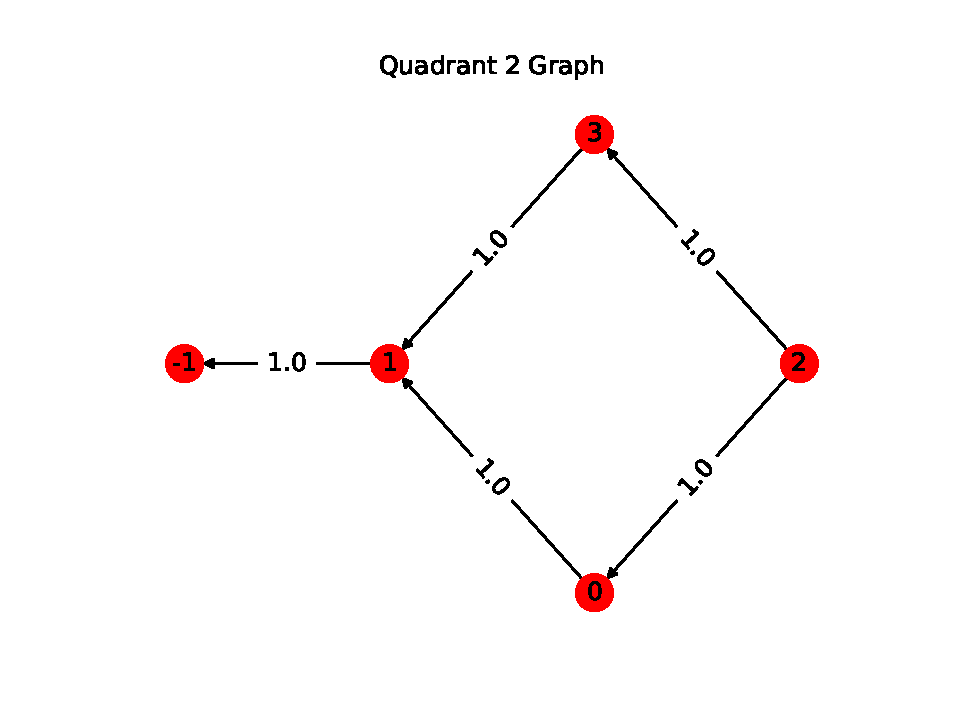
\includegraphics[scale=0.32]{../figures/q2_postweight.pdf}
  \end{minipage}
 
\end{frame}


\end{document}
